\documentclass[pdftex,12pt,a4paper]{book}
\usepackage{ujthesis,enumerate}
\usepackage[nottoc]{tocbibind}
\linespread{1.5}
\dissertation
\coverFont{\large}
\setlength{\spaceLength}{7mm}
\approvedtitle{Particle Swarms and the Frequency Assignment Problem}
\student{William Bezuidenhout}
\degree{Magister Scientiae}
\field{Information Technology}
\faculty{Faculty of Science}
\supervisorName{Dr. G.B. O'Reilly}
\submissionDate{October 2009}
\begin{document}
\makecover
\tableofcontents
\part{Background}
\chapter{Introduction}
\section{Test}
blah blah blah blah
%Introduction
\chapter{Cellular Technology}
\section{Introduction}
In the information age we currently live in almost every device has some sort of wireless technology it uses to provide a specific service. Radios for audio entertainment; Television remotes to change 
channels; Cellular phones for communication; Wireless access points to create wireless LAN's\cite{Karen2004}. Wireless technology is now part of our everyday life.

The popularity and rapid adoption of wireless technology hasn't been kind to the management, planning and operation of wireless networks; It has actually worsen a problem known as the Frequency Assignment problem (FAP) which is present in all forms of wireless communication especially in GSM Cellular networks.

In this chapter we will start of by giving a brief history of the Frequency Assignment Problem. After the brief history overview we will give a description of the problem and explain some of the
underlying concepts needed to understand the Frequency Assignment Problem. We will then move on to discuss the different variants present in the current domain. Further more we will
then discuss the two underlying approaches used in solving the Frequency Assignment Problem (FAP).
\section{GSM Networks}
The General System for Mobile Communications (GSM) is a system for multi-service cellular communication which is capable of providing voice as well as data services. Most cellular networks in operation 
are GSM based. The primary service that GSM caters for is voice communication, but other data services such as Short Message Service (SMS), Multimedia Message Service (MMS) and Internet 
connectivity services such as GPRS are becoming more important\cite{Eisenblatter}.

GSM is one of the most widely used radio communications technologies, which is why we need to look at the history behind it in order for us to understand the domain of radio communication better.We will now present a brief history of the GSM network specification.
\subsection{A Brief History of GSM Networks}
In the early 1981 a group known as the Groupe Speciale Mobile (GSM) was established to develop a Europe wide radio communication system using the reserved 900 MHz band\footnote{In 1990 the United Kingdom requested that 1800MHz band be added to the scope of the GSM standard group. This variant of the GSM specification became known as the \emph{Digital Cellular System 1800} (DCS1800) \cite{GSM92}.}.

At the start of the GSM specification in the early 1980's it was initially thought that the system would be analogue based, but this soon changed with the \emph{Integrated Service Digital Network} (ISDN) specification nearing completetion. As such the GSM specification started following much of the same design principles and access protocols that ISDN exhibited. After the completion of the ISDN specification and the advantages it brought to the field, it became unofficially clear that GSM would be based on digital transmission and that speech would be represented by a digital stream of 16 kbits/s \cite{GSM92}.

Before the switch to digital transmission was finalized the GSM first wanted to evaluate the spectral efficiency of analogue and digital based transmission. Spectral efficiency plays an important part in wireless communication since the radio spectrum is a limited resource and whichever transmission technology is used, should maximise the utilization of the spectrum. Maximum utilisation is an important problem which we will discuss in detail in later sections of this chapter. The Spectral evaluation was conducted over a period of 3 years from 1984-1987. In 1987 a report was published about the 3 year evaluation and subsequently it became official that the GSM system would be digital based using \emph{Time Division Multiple Access} (TDMA) \cite{GSM92,GSMSysEngin}.

By the early 1990’s GSM became an evolving standard and the first GSM based network was demonstrated in 1991\footnote{Near the end of 1991 the GSM group was renamed to \emph{Speciale Mobile Group} (SMG) to eliminate confusion with the standard and the group.}. The following year a number of GSM networks were operating in Europe due to mobile terminals / equipment capable of operating on the networks becoming more widely available to the general public. In the same year an operator in Australia became the first non-European operator to implement a GSM based network\cite{Eisenblatter}.

The collective subscriber base of GSM networks surpassed the million subscriber mark in 1993. Due to this phenomenal growth in GSM network use, numerous extensions were made to the GSM specification. 
Some of the extensions that were made are the following\cite{Eisenblatter}:
\begin{itemize}
\item Half rate speech telephony
\item Improved SMS
\item Line Identification
\item Call waiting
\item Call holding
\end{itemize}
The specification with these extensions defined is known as the GSM Phase 2. As the world shifted towards more digital and data intensive services it became difficult to deliver these services over GSM 
networks. This difficulty was due to the restriction that data could only be transmitted at 9.6 Kbps. A move to eliminate this restriction was made with the specification of GSM Phase 2+. 

The new specification defined new technologies such as General Packet Radio System (GPRS) and \emph{Enchanced Data rate for GSM Evolution} (EDGE) which were designed with the primary goal of making more bandwidth available for data transmission.
These new technologies have an inherent requirement that there be a higher signal to noise ratio present at transceivers. This requirement has an impact that effects radio interfaces and more 
importantly Frequency planning \cite{Eisenblatter}. 

The actual signal to noise ratio at a receiver is dependent on a number of factors that include \cite{Karen2004}:
\begin{itemize}
\item Frequency used at the transceiver
\item Strength of the signal
\item Weather conditions
\item Shape of the surrounding environment
\item Direction of the transmission
\end{itemize}
Even taking these factors into account the calculation of the signal to noise ratio at a transceiver is not trivial. For a more in depth discussion on the calculation the reader is directed at the survey by \cite{Karen2004}.

As the GSM standard matured as a cellular technology, industry experts already began specification of the next generation of cellular networks which would in time, replace the GSM cellular system. The specification of a new standard is considered to be a natural evolution of the technology. Each standard is designed with specific use cases in mind as to what its users might want to do as well as what is possible with the technology at the designers disposal. As time goes by, the technology improves and users habits and needs change, thus the standard must be improved upon to serve these new needs and incorporate new technology.

The \emph{Universal Mobile Telecommunications System} (UMTS) can be considered the 3rd generation (3G) of cellular networks. UMTS was designed from the beginning to operate in parallel with the legacy GSM system. This decision was made to make the deployment of the system as hassle free as possible for the network operators. The first standard of the UMTS was issued in the beginning of 2000 and subsequently most modern networks are based on it or are migrating their networks to it.

UMTS is a large improvement of the GSM in two areas namely Data Transmission bandwidth and Frequency Planning due to UMTS utilising \emph{DS-CDMA} (direct sequence code division multiple access) and \emph{WCDMA} (Wide Band Code Division Multiple Access). The higher data transmission speed (2 Mb/s) can be attributed to UMTS using the DS-CDMA scheme. The scheme also allows more users to be served than previous generation of networks. A direct consequence of WCDMA which sends information over a wide-band of 5 MHz is that no frequency planning problem comparable to that of GSM has to be solved\cite{tabuglobalplanning3g,Eisenblatter}.

In this section we gave a brief overview of the history of the GSM Network specification. In the next section we will present an explanation of the topology of GSM network as well as look at the 
underlying problems present in a GSM networks.
\subsection{Topology of a GSM Network}
GSM networks consists of a variety of different subsystems to realise the goal of establishing a radio communication link between two parties. The hierarchy of systems and their respective connections to
each other is illustrated in figure 1. We will now briefly explain each subsystem.
\subsubsection{Mobile Station (MS)}
A Mobile station (MS) as it is defined in the GSM spec refers to any mobile device that is capable of of making and receiving calls on a GSM network.  The MS is the main gateway 
for a user to gain access to the GSM network. The MS has two features which play an important role throughout the GSM Network, namely:
\begin{description}
\item[Subscriber Identification Module (SIM)] --- Usually inserted into a mobile devices. The SIM contains the \emph{International Mobile Subscriber Identity} (IMSI) and is used throughout the network 
for Authentication as well as being a key part in providing encrypted transmissions.
\item[International Mobile Equipment Identity(IMEI)] --- Used to identify mobile station equipment. Primarily used in the denial of service to equipment that has been blacklisted\footnote{Equipment can be blacklisted for a variety of reasons e.g. theft} and tries to gain access to the network.
\end{description}
The MS has the capability to change the transmission power is uses from its base value to a maximum value of 20 mW. The change in transmission power is automatically set to the lowest level by the Base Transceiver Station to ensure reliable communication after evaluating the signal strength as measured by the MS \cite{GSMSysEngin}. % The power adjustment also minimizes cochannel interference, which we can talk about later when we introduce interference

\subsubsection{Base Station Subsystem (BSS)}

According to the GSM Phase 2+ specification this system is viewed by the \emph{Mobile Switching Centre} (MSC) through an Abis radio interface as the system responsible for communicating with Mobile Stations in a particular location area. The BSS usually consists of one \emph{Base Station Controller} (BSC) with one or more \emph{Base Transceiver Stations} (BTS) which it controls. The communication link between the MSC and BSC is the called the A-interface and the communication link between the BSC and BTS is called the Abis interface. The definition of these communication interfaces is beyond the scope of this disseration, the interested reader is directed to the book \emph{GSM System Engineering} by Asha Mehrotra. A BTS has similar equipment to that of a Mobile Station. Both have transceivers, antennas and the necessary functions to perform radio communication. 

In a GSM network the Service Area (SA) is subdivided into Location Areas(LA's) which are then futher divided into smaller radio zones called cells \cite{GSMSecurInTeleNetwork}. A cell is served by only one BTS and is usually regarded to be in the center of a cell. Even though cells are modelled as being hexagons (See figure 3) the actual coverage area of a cell has no predefined regular shape. Futhermore a cell is divided into 1 to 3 service sectors and each sector is allocated an antenna/transceiver \cite{GSMSysEngin}. Depending on how many sectors are at a cell, the operating angle of the antennae needs to be adjusted accordingly to ensure 360 degree service. If there is only one sector an omni-directional antenna is used, otherwise the antennae operating angle are adjusted to $\frac{360\,^{\circ}}{n}$ where ${n}$ is the amount of antennae \cite{Eisenblatter}.

Each sector operates one or more elementary transceivers called TRX’s. The amount of TRX’s per sector is determined by the expected peak traffic demand that the cell must be able to handle. Each TRX can handle 7 to 8 communication links or calls in parallel except the first TRX, which handles fewer calls than normal due to it being responsible for transmitting cell organisation and protocol information \cite{Eisenblatter}. TRX’s are able to handle 7-8 calls in parallel due to the use of \emph{Frequency Division Multiplexing} (FDM) and \emph{Time Division Multiplexing} (TDM) schemes. TRX’s are assigned channels which enable them to provide conversion between digital traffic data on the network side and the radio communication between Mobile Stations and 
the GSM network. \cite{ACOvsEA,FAPOrientationModel}

\subsubsection{Mobile Switching Centre (MSC)}

The MSC is at the heart of cellular switching system and forms part of the \emph{Network Switching Subsystem} (NSS). The MSC is responsible for the setting up, routing and supervision of calls between GSM subscribers. The MSC has interfaces on the one side to communicate with GSM subscribers (through the BSS) and on the other it has interfaces to communicate with external networks. The MSC interfaces with external networks to utilise their superior capability in data transmission as well as for the signalling and communication with other GSM entities \cite{GSM92}. 

The most basic functions that an MSC is responsibile for in a network are the following \cite{wirelesstelcoMullet}:
\begin{itemize}
\item Voice call initialization,routing,control and supervision between subscribers.
\item Handover process between two cells.
\item Location updating.
\item MS authentication.
\item SMS delivery.
\item Charging and Accounting of services used by subscriber.
\item Notification of other network elements.
\item Administration input or ouput processing functions.
\end{itemize}

To achieve most of these functions the MSC has an integrated \emph{Visitor Location Register (VLR)} database that stores call setup information for any MS that is currently registered for service with the MSC \cite{GSM92,wirelesstelcoMullet}. 

The VLR retrieves this information from the \emph{Home Location Register (HLR)} which contains all the registered GSM subcriber information for the network. This information enables the MSC to quickly retrieve the nesaccery information to setup a call between two entites \cite{GSMSysEngin,GSMSecurInTeleNetwork}.

A requirement for being able to communicate with other network elements such as \emph{Public Switching Telephone Networks} (PSTN) is the ability to multiplex and demultiplex signals to and from such network elements. This operation is a necacity, since the incoming or outgoing connection bitrate from the source entity might either be to low or to high for the receiving entity.

A typical scenario where this operation proves vital is when a mobile subcriber makes a call to a subcriber on a PSTN. The connection bit rate needs to be changed at the MSC from a wireless connection bitrate to a bitrate suitable for transmission over a PSTN.

\subsubsection{Network Databases}
The HLR, AUC (Authentication Center) and EIR (Equipment Identity Register) are the 3 'back-end' databases which stores and provides information for the rest of the GSM Network. We will now briefly discuss what the purpose of each database is and its core functions.

\paragraph{Home Location Register (HLR)}
The HLR is a database that permenantly stores information pertaining to a given set of subscribers. The HLR needs to store a wide range of subcriber parameters because it is the reference source for anything GSM subscriber related in the network. 

Subscriber parameters that are stored in the database include: Billing information, routing information, identification numbers, authentication parameters,subscribed services. The following information is also stored but the information is of a temporary nature and can change at anytime: Current VLR and MSC the subscriber is registered with; Wheter the subscriber is roaming \cite{GSMSysEngin}.

\paragraph{Authentication Center (AUC)}
The Authentication center is the entity in the GSM network that performs security functions and thus stores information that enables it to provide secure over the air communication. The information that is stored contains authentication information as well as keys that are used in ciphering of information.

During an authentication procedure no ciphering key is ever transmitted over the air, instead a challenge is issued to the mobile who needs to be authenticated. This callenge requires the mobile station to provide the correct \emph{Signed Response}(SRES) with regard to the random number generated by the AUC. The random number and ciphering keys that are used change with each call that is made, thus an attacker would gain nothing by intercepting a key, since it will change with the next call \cite{GSMSysEngin}.

Each mobile that is registered in the HLR database needs to be authenticated and each call that is instansiated needs to retrieve keys from the AUC to establish a secure communication link. The AUC is sometimes included with HLR to allow for fast communication between the two entities \cite{GSMSysEngin}.

\paragraph{Equipment Identity Register (EIR)}
The EIR is a database that stores the IMEI numbers of all registered mobile equipment that has accessed the network. Only information about the mobile equipment is stored, nothing about the subscriber or call is stored in the database.

Typically there is only one EIR database per network and interfaces to the various HLR database contained in the network. The IMEI's are grouped into 3 categories: \emph{White List}, \emph{Black List} and the \emph{Gray List}. The White list contains only the IMEI numbers of valid MS's; the Black List stores the IMEI numbers of equipment that has been reported stolen and the Gray List stores the IMEI numbers of equipment that has some fault (faulty software, wrong make of equipment).

\subsubsection{GSM Network Management entities}
In a GSM network most of the elements that form part of and make the network function are often distributed in a wide geographical area to provide the best network converage for the customer. 

For a network to function properly and efficiently network engineers need to be kept up to date on the state of the network and be alerted if \emph{any} problems occur. For this purpose there exists two systems in the GSM network architecture that allows for this functionality required by network engineers. 

The one system is called the Operations and Management center which is responsible for centralized regional and lcoal operational and maintenance activities. The other system called the Network Management System unlike the OMC provides global and centralized managemenent for operations and maintenance of the network suppored by the OMCs \cite{GSMSysEngin}.

We will not discuss the OMC and NMC in a bit more detail where we'll define the most critical functions they peform.

\paragraph{Operational and Managemenet Center}
The OMC is capable of communicating with GSM entities using two protocols namely SS7 and X.25. The SS7 protocol is usually used when the OMC is communicating within the GSM network over short and medium distances. The X.25 protocol is used for large external data transfers. All communication where the OMC is involved typically occurs over fixed line networks and/or leased lines. The OMC is usually used for day to day operation of a network \cite{GSMSysEngin}.

The OMC has support for alarm handling. An alarm in a GSM network goes of whenever a predefined expected condition does occurs. Engineers are able to define the severity of an alarm which defines who and what is futher alerted when and if the alarm is escalated to a higher level \cite{GSMSysEngin}.

To give one an idea of when and why and alarm goes of consider the following scenario: The MSC controls a set of BSS systems. Now for some reason a certain region experiences a power blackout. All the BSS affected by the blackout switch over to reserve power if availble. A first alarm is sounded to let the engineers / network know that the BSS is using reserve power. When the BSS reserve power is depleted the MSC sounds an alarm letting the network know that a specific BSS cannot be contacted.

Typically in the above scenario the severity of the first alarm will be of a medium priority. The second alarm is much more serious and its severity will be of a high priority.

The OMC is also capable of fault management in the GSM network. The OMC is able to activate,deactivate,remove and restore a service manually or automatically of network devices. Various tests can be run as well as diagnostic information can be retrieved on the network devices to detect any current or future defects \cite{GSMSysEngin}.

\paragraph{Network Management Center}
The NMC is similar to the OMC but it is not restricted to only regional GSM entities as it is in charge of the all GSM entities in the network. The NMC provides traffic management for the global network and also monitors high priority alarms such as overloaded or failed network nodes. It is usually used in long term planning of a network, but it has the capability to perform certain OMC functions when an OMC is not staffed. 

\subsection{GSM Network problems}
\section{The Frequency Assignment Problem}
The Frequency Assignment Problem (FAP) is a generalisation of the graph-colouring problem and is subsequently an NP-hard problem. This is because one has a finite amount of frequencies which needs to be 
assigned to antennae/transceivers (TRX's)  where the amount of transceivers to be assigned frequencies greatly out weigh the amount of available frequencies. Thus it is inevitable that a network will 
have interference and we can only minimise the amount of interference that might occur on the network - an optimisation problem. 

A contributing factor to the difficulty of the FAP is due to the scarcity of usable frequencies in the radio spectrum, which forces network operators to reuse their allocated/licensed frequencies in their respective networks. The scarcity of the usable frequencies in the spectrum can be attributed to the overuse of certain bands as well as large scale reuse of frequencies in networks. This has put strain on the spectrum and has complicated the management of networks significantly because interference is more likely to occur.

\subsection{Interference}
Interference occurs when frequencies assigned to connections differ by a small margin. The amount of inference on a connection defines the quality of service. One can naturally make the deduction that 
the more frequencies differ used on connections in a area, the better quality of service one will experience in that area. Cellular networks use the amount of interference on their networks as 
qualitative measure for their \emph{Quality of Service} (QoS). A network with high interference would experience a lot of dropped connections, which occurs when the interference is too high to sustain a connection for communication.

Primarily Interference occurs if the Electromagnetic constraints are violated, which are defined as:
\begin{description}
\item[Co-Cell] ---
\item[Adj Channel] ---
\item[Co-Site] ---
\end{description}
A fourth constraint, namely the Handover constraint is also applicable in Cellular networks which we will discuss in section 4.

\subsection{Frequency Assignment Types}
Within the FAP domain there are  a variety of sub problems which originated over the decades of which wireless communication has survived through. We will discuss the most popular problems found in the literature over the last few years in Section 2. The FAP can be classified into two categories:
\begin{enumerate}[\bf{(}a\bf{)}]
\item \emph{Fixed Frequency/Channel Assignment} (FFA/FCA) is the process of permanently assigning frequencies to cells (cellular towers). The frequencies assigned are fixed and cannot be changed on the fly while 
the network is active , since the frequencies assigned to the cell form part of a delicate frequency plan designed to keep interference to minimum.
\item \emph{Dynamic Frequency/Channel Assignment} (DFA/DCA) is the process of allocating channels to cells as they require it to meet the current traffic demand imposed on them by clients. 
\end{enumerate}
Each cell can be assigned multiple frequencies based on the amount of transmitters or TRX's it has. The amount of TRX's in a cell depends on the expected amount of traffic the particular cell must 
handle.

Most of the research in the FAP has concentrated on the FFA. The reason for this is because FFA is a static technique, which allows it to come up with a better solution since it has more time for 
calculation. FFA is also easier to implement in practise and allows the network operators to cater for the worst case scenario - heavy traffic load on the network. The DFA is at the moment a very hard 
problem because the network frequency plan is constantly changing, which means as the traffic on the network increases the longer the DFA focused algorithm will take to allocate a frequency. This 
increase in processing time is because the algorithm has to take into account more constraints with a lower available frequency pool. DFA must do this process within seconds since a cell needs to serve clients. Most researchers have concentrated on solving the FFA using heuristic approaches like neural networks, local search techniques and more recently meta heuristic approaches which include genetic algorithms, simulated annealing , ant colony optimisation and particle swarm optimisation.

In this section we have given a description of the Frequency Assignment Problem and introduced some concepts which we will use throughout the dissertation. In the next section we will present the 
Mathematics that govern the Frequency Assignment Problem.
\subsection{Mathematical Formulation}
\subsection{Types of Frequency Assignment Problems}
\subsubsection{Minimum Order Frequency Assignment Problem}
\subsubsection{Minimum Span (MS) Frequency Assignment Problem}
\subsubsection{Fixed Spectrum (FS) Frequency Assignment Problem}
\subsection{Frequency Assignment Models}
\subsubsection{Binary Constraints}
\subsubsection{Cost Function Minimisation}
\section{Summary}
%The Frequency Assignment Problem
\chapter{The Frequency Assignment Problem}
\section{Introduction}
The Frequency Assignment Problem (FAP)\footnote{Also known as Automatic Frequency Planning (AFP) or Channel Assignment Problem (CAP)\cite{ACOvsEA}} is a generalisation of the graph-colouring problem and is subsequently an NP-hard problem. This is because one has a finite amount of frequencies which needs to be assigned to antennae/transceivers (TRX's)  where the amount of transceivers to be assigned frequencies greatly out weigh the amount of available frequencies.

It is inevitable that a network will have interference and we can thus only minimise the amount of interference that might occur on the network - an optimisation problem. Using exact algorithms to find a solution is not practical since the time to find a solution will be polynomial. Generally Metaheuristic algorithms are used to find optimal solutions to NP-hard problems\cite{ACOvsEA}. We will discuss Metaheuristic algorithms which are generally used to find solutions for NP-hard problems in Chapter 4. 

A contributing factor to the difficulty of the FAP is due to the scarcity of usable frequencies in the radio spectrum, which forces network operators to reuse their allocated/licensed frequencies in their respective networks. The scarcity of the usable frequencies in the spectrum can be attributed to the overuse of certain bands as well as large scale reuse of frequencies in networks. This has put strain on the spectrum and has complicated the management of networks significantly because interference is more likely to occur.

Frequency assignment is the last step in a long process of network setup. Before frequencies are assigned base stations need to be placed and need to be configured, which include azimuth and tilt of the antenna for optimal network coverage. After the base stations are configured they need to be allocated a certain amount of transmitters to achieve a target network capacity \cite{AndreasPaper}.

Frequency assignment is only a means to achieve the targeted network coverage as well as network capacity.

In this section we gave a brief introduction as to what the Frequency Assignment Problem is and why it occurs as well as why it is a problem. In the next section we will describe the types of Frequency Assignment in use today and we will also discuss some of the varaints of FAP and also formally define which of the variants we will concentrate on.
\section{Frequency Assignment Types}
In this section we will discuss the different methods that exist to allocate frequencies to cells in a cellular network. We will also state which method we will use through out this paper.

Within the FAP domain there are  a variety of sub problems which originated over the decades of which wireless communication has survived through. We will discuss the most popular problems found in the literature over the last few years in Section 2. The FAP can be classified into two categories:
\begin{enumerate}[\bf{(}a\bf{)}]
\item \emph{Fixed Frequency/Channel Assignment} (FFA/FCA) is the process of permanently assigning frequencies to cells (cellular towers). The frequencies assigned are fixed and cannot be changed on the fly while the network is active , since the frequencies assigned to the cell form part of a delicate frequency plan designed to keep interference to minimum.
\item \emph{Dynamic Frequency/Channel Assignment} (DFA/DCA) is the process of allocating channels to cells as they require it to meet the current traffic demand imposed on them by clients. 
\end{enumerate}
Each cell can be assigned multiple frequencies based on the amount of transmitters or TRX's it has. The amount of TRX's in a cell depends on the expected amount of traffic the particular cell must 
handle.

Most of the research in the FAP has concentrated on the FFA. The reason for this is because FFA is a static technique, which allows it to come up with a better solution since it has more time for 
calculation. FFA is also easier to implement in practise and allows the network operators to cater for the worst case scenario - heavy traffic load on the network. The DFA is at the moment a very hard 
problem because the network frequency plan is constantly changing, which means as the traffic on the network increases the longer the DFA focused algorithm will take to allocate a frequency. This 
increase in processing time is because the algorithm has to take into account more constraints with a lower available frequency pool. DFA must do this process within seconds since a cell needs to serve clients. Most researchers have concentrated on solving the FFA using heuristic approaches like neural networks, local search techniques and more recently meta heuristic approaches which include genetic algorithms, simulated annealing , ant colony optimisation and particle swarm optimisation.

In this section we have given a description of the Frequency Assignment Problem and introduced some concepts which we will use throughout the dissertation. In the next section we will present the 
Mathematics that govern the Frequency Assignment Problem.
\section{Interference}
In this section our disuccsion will focus on Interference. We will describe what interference is and why it is important for cellular networks as well as give an overview of when interference occurs.

Interference occurs when frequencies assigned to connections differ by a small margin. The amount of inference on a connection defines the \emph{Quality of Service} (QoS). One can naturally make the deduction that the more frequencies differ used on connections in a area, the better quality of service one will experience in that area. 

Cellular networks use the amount of interference on their networks as qualitative measure for their QoS. A network with high interference would experience a lot of dropped connections/calls, which occurs when the interference is too high to sustain a connection or call for communication, consequently their QoS degrades as interfernece increases.

In the literature a variety of methods are given to calculate the amount of interference in a network. These methods range from theoretical approaches to precise measurements. Regardless of what method is used the end result which they all produce is called an \emph{Interference Matrix} denoted as \emph{M}\cite{ACOvsEA}.

An Interference Matrix concists of a number of cell pairs (\emph{i,j}), where \emph{i} is the cell receiving interference and \emph{j} the cell whose allocated channel is providing the interence. Each cell pair in the matrix has two corresponding values that indicate the level of interference if the \emph{Electromagnetic constraints} are violated \cite{Eisenblatter,Karen2004,ACOvsEA}. These values are usually normalized to be between 0.0 and 1.0 \cite{AndreasPaper}.

Primarily Interference occurs when the Electromagnetic constraints are violated, which are defined as:
\begin{description}
\item[Co-Channel] --- When a cell \emph{i} and a cell \emph{j} operate on the same frequency or channel interference will occur \cite{Eisenblatter,EfficientEvoChannelManagement,Karen2004,ACOvsEA,InterferenceOrientatedFAP}. This is called co-channel interference. This constraint is the most important constraint that must not be violated to ensure proper performance and reliability of a modren cellular network\cite{EfficientEvoChannelManagement}.
\item[Adjacent Channel] --- When a cell \emph{i} and a cell \emph{j} operate on adjacent channels, their allocated frequencies differ by one i.e. cell \emph{i} operates on channel \emph{f} then if cell \emph{j} operates on either channel \emph{f - 1} or \emph{f + 1} then adjacent channel interference will occur \cite{Eisenblatter,EfficientEvoChannelManagement,Karen2004,ACOvsEA,InterferenceOrientatedFAP}
\item[Co-Site] --- If cell \emph{i} and cell {j} are located at the same site, then their allocated frequency ranges must differ by a certain distance in the frequency domain. This distance is known as the reuse distance \cite{FixedFAPPSO,EgyptFAPPSO}.
\end{description}
A fourth constraint, kown as the Handover constraint, is also applicable in Cellular networks. This constraint imposes a separation in frequencies when one cell hands over a call to another cell. If this constrain is violated a mobile subscriber will experience a dropped call since the handover between cells fials.The above constraints only account for factors that are in our control.

Interference also occurs due to techincal limitations, natural phenonema and other external factors like other systems. Thus another constraint is imposed on the frequency that is allocated to cell. This constraint is known as the \emph{separation} constraint which imposes a minimum separation between frequencies assigned to a cell \cite{Eisenblatter,InterferenceOrientatedFAP}. To avoid clashes with other operator frequencies each cell may also have a set of locally forbidden frequencies which are not allowed to be used under any circamstance.

In this section we described what interfenece is and what the consiquences are of too much interfence in a network. We also laid out under which circumstances interference can occur in a cellular network. In the next section we will give a Mathematical Formulation of the Frequency Assignment Problem.
\section{Types of Frequency Assignment Problems}
\subsection{Minimum Order Frequency Assignment Problem (MO-FAP)}
\subsection{Minimum Span Frequency Assignment Problem (MS-FAP)}
\subsection{Minimum Interference Frequency Assignment Problem (MI-FAP)}
\section{Fixed Spectrum MI-FAP Mathematical Formulation}
In this section we will give a Mathematical definition of the Frequency Assignment Problem which will form the core of what our algorithm discussed in this paper will optimize. We'll start of by denoting the symbols we will use and then we will give the Mathematical definition of the cost function we will try to minimize using our denoted symbols.

Let \((V,E)\) be an undirected graph called \(G\) with vertex and edge labelings. A vertex is introduced for each transmitter or carrier representing the TRX. An edge for every interdependency between corresponding transmitters. The spectrum \(C\) is an interval in the frequency domain.The traffic demand requirement is denoted by a \(n\)-element vector represented by \(d\). Each element \(d_i\) represents the amount of channels to be assigned to cell \(i\).

There are three types of interdependencies recorded between transmitters with edge labels.
\begin{enumerate}
\item \emph{Seperation} --- \(d(vw) \subseteq \{0,1,2,3\}\) is the minimum required difference of the channels assigned to \(v\) and \(w\).
\item \emph{co-channel interference} --- \(c^{co} (vw) : E \rightarrow [0,1]\) where E denotes the amount of interference incurred if the same channel is allocated to \(v\) and \(w\).
\item \emph{adj-channel interference} --- \(c^{adj} (vw) : E \rightarrow [0,1]\) where E denotes the amount of interference incurred if the channel allocted to \(v\) and \(w\) violated the adjacent channel constraint.
\end{enumerate}

Let \(M = \lbrace (c^{co} (vw),co^{adj} (vw))\rbrace\) be a given matrix called the interference matrix.

In this section we Mathematically defined the Frequency Assignment Problem using the symbols we defined. In the next section we will give a brief discussion on the different Frequency Assignment Problems that exist and also define the the problem we will concentrate on through the rest of this disseration.
\section{FAP Benchmarks}
\paragraph{Philledelphia Benchmark}
\paragraph{Calma Project}
\paragraph{COST 256}
\section{FAP in the industry}
\paragraph{Satelite communication}
\paragraph{Wireless mesh networks}
\paragraph{Military field communication}
\paragraph{Media Broadcasting}
\paragraph{Cellular Communication}
\section{Summary}
%Metaheuristics
\chapter{Metaheuristics and the Frequency Assignment Problem}
\section{Introduction}
%Metaheuristics and the Frequency Assignment Problem
\chapter{Swarm Intelligence}
\label{chpt:swarm}
\section{Introduction}
The research field of Artificial Intelligence stands a lot to gain by studying the underlying inner workings of nature itself; this is why there is a branch of Artificial Intelligence that incorporates some of natures processes, like genetics, which can be seen being applied in practice in the genetic algorithm (see section \ref{sec:geneticalgorithm} page \pageref{sec:geneticalgorithm}).

 There are other approaches in Artificial Intelligence which also have their routes in nature, like for instance animal learning or the study of how dogs learn\cite{DLearning}. These approaches only look at a “single agent” thought process when it maps percepts (senses) to actions in its respective environment \cite{DLearning}. 
 
 A percept can be said to be a process that is specifically designed to take data from the surrounding environment, process it and present it as information upon which decisions can be made\cite{DLearning,AIModernApproach}. For instance, eyes are percepts, which take visual data presented by the environment\cite{DLearning,AIModernApproach}. The visual data is processed by the brain into information to enable decisions to be made on navigating the environment\cite{DLearning,AIModernApproach}.

The research field of swarm intelligence is an approach more concerned with the underlying processes and behaviour patterns when multiple agents (insects, animals) come together and perform a task as one collective entity\cite{DLearning,AIModernApproach,ChaoticSwarmIntel,BeeJobShop}.  This study of animals or insects in groups has already contributed to Artificial Intelligence as a whole \cite{ChaoticSwarmIntel,BeeJobShop}. Each individual in the swarm might not be able to solve the problem on his own, but by interacting with other individuals and performing primitive actions, the individual can contribute to solving the problem as a whole entity \cite{BeeJobShop}. 

New algorithms that incorporate the lessons learned from the study of the collective intelligence are now being used and form part of the Meta-heuristic algorithm group. A discussion on some of the more popular meta-heuristic algorithms was presented in chapter~\ref{chpt:heuristic} (see page~\pageref{chpt:heuristic}).

Swarm intelligence algorithms are also meta-heuristic algorithms, with the distinction being made that swarm intelligence algorithms use multiple agents as a collective entity of knowledge to search the problem space\cite{SwarmArt,ChaoticSwarmIntel,BeeJobShop,CompuIntelligenceIntro,FundamentalSwarm}.

The initial algorithms developed with regard to swarm intelligence, where based on the coordination and behaviour exhibited by schools of fish and flocks of birds. The newer generation of algorithms include\cite{SwarmArt,ChaoticSwarmIntel,BeeJobShop}:
\begin{itemize}
\item Ant Colony Optimization\cite{SwarmArt}.
\item Artificial Bee Colony Optimization\cite{BeeJobShop}.
\item Particle Swarm Optimization\cite{ChaoticSwarmIntel}. 
\end{itemize}

These newer generations of algorithms are primarily being used in combinatorial NP-Complete problems, where there is no defined solution, only an optimization that comes close to an optimal solution. Swarm intelligence works on a key feature observed in nature, the notion of emergent behaviour\cite{SwarmArt,CompuIntelligenceIntro,FundamentalSwarm}. Whenever an entity does something unconventional and gains success, it can be considered as exhibiting “emergent behaviour” as if it is emerging out of the masses way of doing things\cite{SwarmArt,CompuIntelligenceIntro,FundamentalSwarm}. 

Typical emergent properties exhibited by swarms are self-organization and synchronization \cite{SwarmArt}. In swarm intelligence, when an agent exhibits emergent behaviour, the behaviour of the agent needs to be shared to the whole swarm, in order for the swarm to adapt and use the newly gained knowledge\cite{SwarmArt,ChaoticSwarmIntel,CompuIntelligenceIntro,FundamentalSwarm}.

The information that is shared among the individuals of the swarm can be anything that contributes to the swarm as a whole, like for instance the information might be about a new solution that is better than all previous solutions \cite{SwarmArt,ChaoticSwarmIntel,CompuIntelligenceIntro,FundamentalSwarm}. 

The behaviour propagates from one agent to another through social interaction, which brings forth information exchange\cite{SwarmArt}. Social interaction is but one component of self-organization. Other components that form part of self-organization are \cite{SwarmArt}:
\begin{itemize}
\item Positive and negative feedback
\item Increasing the magnitude of fluctuations
\end{itemize}

Individuals within swarm are able to accomplish social interaction with each other to achieve information sharing by using a concept referred to as \emph{stigmergy}\cite{SwarmArt,CompuIntelligenceIntro,FundamentalSwarm}. A discussion on stigmergy as well as the different forms of stigmergy that exist will be discussed in section~\ref{sec:stigmergy}.

Utilizing stimergy along with self-organization swarm intelligence algorithms like Ant Colony Optimization, Particle Swarm Optimization and Artificial Bee Colony Optimization are able to produce relatively good results for NP-Complete problems\cite{CompuIntelligenceIntro,FundamentalSwarm,SwarmArt}. 

Swarm intelligence based algorithm are able to achieve this since they have small individuals searching for more optimal values for a potential optimal solution on multiple fronts. As one individual makes progress on a certain front, its knowledge is shared\cite{CompuIntelligenceIntro,FundamentalSwarm}. 

With traditional single agent based meta-heuristic algorithms like Tabu Search (section~\ref{sec:tabusearch} page~\pageref{sec:tabusearch}) and Simulated Annealing (section~\ref{sec:simulatedannealing} page~\pageref{sec:simulatedannealing}) only have in essence one "individual" searching for a solution\cite{CompuIntelligenceIntro,FundamentalSwarm}. 

With algorithms like TS and SA, the information is not shared since there is nothing to share it with due to only one individual search\cite{CompuIntelligenceIntro,FundamentalSwarm,SASingleMultiObj,TSHazardous}. The information is kept to influence future decisions\cite{AIModernApproach,TabuMontemanniSmith,TabuVechicleRoutingWithTimeWindows,CurveFittingSA,EcoEquilSA}. Swarm Intelligence algorithms also store information for use by the various individuals that make up the swarm to make more informed decisions as the solution space is explored\cite{CompuIntelligenceIntro,FundamentalSwarm}.

NP-Complete\footnote{Discussion on NP-Complete problems is presented in section~\ref{sec:NPComplete} page~\pageref{sec:NPComplete}} optimization problems is but only one of the fields of applicability where swarm intelligence algorithm have been applied. Other fields where swarm intelligence has been applied include neural network training\cite{CompuIntelligenceIntro}, vehicle routing\cite{ACOSurvey}, clustering\cite{AntSwarmClustering}, search engines and electrical power systems\cite{SAElectricPower}. Swarm Intelligence thus seems more suited towards problems with combinatorial complexity\cite{SIOPDenby}.

In this chapter the first discussion will be on the Ant Colony Optimization in section~\ref{sec:ACO}. Particle Swarm Optimization will be discussed in section~\ref{sec:PSO}. This chapter will conclude with section~\ref{sec:BEE} where a discussion on the Bee Colony Algorithm will be presented. 

Before the algorithms are discussed. A small overview on stigmergy will be given, as it forms a core concept upon which swarm intelligence algorithms are based upon.
\section{Stigmergy}
\label{sec:stigmergy}
Stigmergy is defined as the method animals and insects use to facilitate communication through interaction\cite{AntsAndStigmergy,CompuIntelligenceIntro,AntIntroTrends,FundamentalSwarm}. Through the use of stimergy animals or insects are able to socially interact with their own species to convey information to each other\cite{AntsAndStigmergy,CompuIntelligenceIntro,AntIntroTrends,FundamentalSwarm}.

Interaction occurs through signals that the individuals receive which might require them to perform a specific action\cite{AntsAndStigmergy,CompuIntelligenceIntro,AntIntroTrends}.

Two forms of stigmergy can be observed in nature. The one form, \emph{Sematectonic stigmergy}\label{def:sematectonic}, is a direct and physical form of interaction since it relies on altering the environment or by using some for of physical action to communicate \cite{CompuIntelligenceIntro}. 

Examples of this type of stigmergy being used include nest building and brood sorting by ants\cite{CompuIntelligenceIntro}. Schools of fish also use this type of stigmergy to communicate direction and speed by visually observing their closest partner in the school. Besides using visual information, birds use sound to communicate and alert each other\cite{SwarmArt}.

The other form, \emph{Sign-based stigmergy} is an indirect form of interaction, where communication occurs through some sort signal mechanism\cite{CompuIntelligenceIntro}. Ants use sign-based stigmergy to communicate with each other. More on how ants communicate with this type of stigmergy will be discussed in section~\ref{sec:ACOverview}.

Other species that use sign-based stigmergy are bees\cite{stigmergicoptimization}. When a bee determines that entity poses a threat to the hive, the bee might decide to sting the entity. The sting of a bee not only injects a toxin into the entity, but also releases a pheromone\cite{stigmergicoptimization}. This pheromone alerts nearby other bees from the hive of the presence of entity that is a potential danger to the hive\cite{stigmergicoptimization}. 

The other bees of the hive pick up this pheromone that is released by the initial bees stinger and therefore attacks the entity by also stinging it\cite{stigmergicoptimization}. As more bees sting the entity, more bee stingers emit the danger pheromone identifying the entity\cite{stigmergicoptimization}. Hence the pheromone gets reinforced and thus stronger which persuades more bees into action\cite{stigmergicoptimization}.

Stigmergy is a powerful mechanism that is able to alter the behaviour of a collective entity efficiently, as can be gathered from the above mentioned examples of where stigmergy is used in nature\cite{AntsAndStigmergy,CompuIntelligenceIntro,AntIntroTrends}. Stigmergy is therefore a core concept upon which Swarm Intelligence algorithms are based as these communication techniques are exploited to aid the algorithm in finding better solutions\cite{AntsAndStigmergy,CompuIntelligenceIntro,AntIntroTrends}.

In the forth coming sections three swarm intelligence algorithms will be discussed. Each section is divided into four subsections. 

First, an overview of the algorithm will be given, where basic concepts about the algorithm will be discussed as well as a general outline of the search process the algorithm uses. 

The second subsection will provide a step by step discussion of the algorithm using presented pseudo code as reference.

The third subsection will give an in depth discussion on some of the core characteristics that make the algorithm unique. 

Finally, for each algorithm discussed a subsection will be presented where literature using the algorithm on the FAP is presented as well as description of the various considerations one needs to make to apply the algorithm on the FAP.

\section{Ant Colony Optimization (ACO)}
\begin{algorithm}
\caption{Basic Ant Colony Optimization Algorithm~\cite{CompuIntelligenceIntro}}
\label{alg:ACO}
	\begin{algorithmic}[1]
	\STATE$\text{Initialize $\tau_{ij}$ with small starting values}$
	\STATE$t \leftarrow 0$
	\STATE$\text{Place $n_k$ ants on starting node}$
	\WHILE{stopping condition not reached}
		\FOR{each ant $k \leftarrow 0$ to  number of ants $n_k$}
			\STATE$p^k(t) \leftarrow \text{Initialize path } p^k \text{for time step } t$
			\REPEAT
				\STATE$\text{Select next node based on probability equation~\ref{eq:ASprobability}}$
				\STATE$\text{Add link (i,j) to path } p^k(t)$
			\UNTIL{Final node reached}
			\STATE$x^k(t) \leftarrow \text{Remove loops from path }p^k(t)$
			\STATE$\text{Calculate length of path $f(p^k(t)$})$
		\ENDFOR
		\FOR{each link $(i,j)$ in graph}
			\STATE$\tau_{ij} = \text{Reduce pheromone of link $(i,j)$ with equation~\ref{eq:pheromoneevapuration}}$
		\ENDFOR
		\FOR{each ant $k = 0$ to  number of ants $n_k$}
			\FOR{each link $(i,j)$ in $p^k(t)$}
				\STATE$\triangle \tau_{ij} = \frac{1}{f(p^k(t))}$
				\STATE$\text{Update the pheromone $\tau_{ij}$ with equation~\ref{eq:pheromoneupdate}}$
			\ENDFOR
		\ENDFOR
		\STATE$t \leftarrow t + 1$
	\ENDWHILE
	\RETURN $\text{path $x^k(t)$ with the smallest $f(x^k(t))$ as the solution}$
	\end{algorithmic}
\end{algorithm}
\label{sec:ACO}
\begin{figure}[p]
	\begin{center}
	\fbox{\includegraphics[width=5.0in,height=5.5in]{./pictures/AntColonyOptimization.pdf}}
	\caption{Flow Chart for ACO Algorithm}
	\label{fig:ACOAlgorithmFlowChart}
	\end{center}
\end{figure}
\subsection{Introduction}
\label{sec:ACOverview}
Ant Colony Optimization (ACO) is a class of algorithms incorporating different behavioural aspects that ants exhibit when they perform certain activities i.e. gather food, build nests and construct cemeteries\cite{AntsAndStigmergy,CompuIntelligenceIntro}. The first ACO algorithms that were developed were based on the foraging behaviour that was exhibited by ants when finding the most optimal path towards a food source. Deneubourg noticed the foraging behaviour when he performed the Bridge experiment \cite{AntsAndStigmergy,CompuIntelligenceIntro}.
\begin{figure}[b!]
	\centering
	\setlength \fboxsep{0pt}
	\setlength \fboxrule{0.5pt}
	\fbox{\includegraphics[width=4.0in,height=2.0in]{./pictures/antBridgeExperiment.png}}
	\caption{The Ant bridge experiment \cite{AntsAndStigmergy}}
	\label{fig:antBridgeExperiment}
\end{figure}

Deneubourg wanted to know how ants where able to find the shortest path towards a food resource and communicate it to the whole nest \cite{AntsAndStigmergy}. Thus an experiment was setup up to study the ants' behaviour. In the experiment a food source was placed a certain distance away from the nest\cite{AntsAndStigmergy,CompuIntelligenceIntro}. Two paths were setup towards the food resource, one path was purposely made longer than the other path as can bee seen in figure \ref{fig:antBridgeExperiment} \cite{AntsAndStigmergy}.

Ants would exit the nest in order to forage food\cite{AntsAndStigmergy,CompuIntelligenceIntro}. The ants first started exploring the area outside the nest in an attempt to locate a suitable food source\cite{AntsAndStigmergy,CompuIntelligenceIntro}. As the ants in the experiment explored the immediate space outside the nest to the food source, they had to take one of the provided paths to the food source\cite{AntsAndStigmergy}.

The ants initially oscillated between the paths with no clear distinction of the more dominant route to take to retrieve food from the food source\cite{AntsAndStigmergy,CompuIntelligenceIntro}. After a certain amount of time the one path to the food source became the preferred route for the ants as the specific path was indeed the shortest path towards the food source \cite{AntsAndStigmergy}.

Naturally the questioned that was asked was how were the ants able to communicate to each other that the one food source was closer than the other? The answer lies in the use of \emph{stigmergy} by ants\cite{AntsAndStigmergy,CompuIntelligenceIntro}. Ants use sign-based stigmergy (discussed in section~\ref{sec:stigmergy}) when they retrieve food\cite{AntIntroTrends,AntsAndStigmergy,CompuIntelligenceIntro}. As the ant moves along a particular path, it marks the path with a chemical signal that alerts other ants to the desirability of the path \cite{CompuIntelligenceIntro}. The chemical signal that ants use to indicate optimal paths is called \emph{pheromones}\cite{AntsAndStigmergy,CompuIntelligenceIntro}.

A path is made up of a series of links between nodes\cite{AIModernApproach,DataStructuresJava}. A link between two nodes represents a movement from the one node to the other\cite{AIModernApproach,DataStructuresJava}. Therefore, a path can be considered as the traversal of the interlinked nodes, from a starting node to some final node\cite{AIModernApproach,DataStructuresJava}. A path differs from another path by the order in which the nodes are interlinked between a start and end node\cite{AIModernApproach,DataStructuresJava}.


The concept of pheromones and how the ACO goes about in updating the pheromones is a critical concept of ACO hence, an in depth discussion on pheromones will be provided in subsection \ref{sec:ACOcharacter}.

The ACO algorithms are considered stochastic search procedures due to their innate use of randomness when exploring the solution space \cite{ACOSurvey,ImpACOComplex}. The ACO class of algorithms has been applied to a wide range of problems that include --- Single Machine Scheduling\cite{ACOSingleMachine},Weapon target assignment\cite{WeaponTargetACO}, Flow shop scheduling\cite{ACOFlowShop} and Image Thresholding\cite{ACOImageThreshold}. Various variants of the standard algorithm have been developed but all of the algorithms sill follow the basic structure listed in algorithm~\ref{alg:ACO}\cite{CompuIntelligenceIntro,FundamentalSwarm}.

The ACO algorithm have achieved relatively good success of the problems it has been applied, but does have some disadvantages\cite{ImpACOComplex,ACOSurvey}. One of the primary disadvantages of ACO is that it tends to get stuck on local minima in the solution space therefore, the solution space isn't adequately explored and the algorithm prematurely converges to a local optima \cite{ImpACOComplex}.

To combat the shortcoming of getting stuck in local optima, the MAX-MIN Ant Optimization algorithm was developed. The MAX-MIN algorithm is based on the original Ant system algorithm. MAX-MIN addresses the local minima problem by imposing dynamically changing bounds on the pheromones of the ants such that it is always falls within the limit of the heuristic and best current path of the colony\cite{GangWangACO}.

The first algorithm to be based on the behaviour of ants was called the Ants System (AS) \cite{CompuIntelligenceIntro,AntIntroTrends}. The AS was initially applied to the Traveling Salesman problem (TSP) as a proof of concept but its performance on TSP was lacklustre compared to other algorithms applied to the same problem \cite{CompuIntelligenceIntro,AntIntroTrends}. 

Subsequently, various algorithms have been developed that improve on the AS algorithm. These improved algorithms include the Ant Colony System (ACS), The ANTS system, Ant-Q and AntTabu \cite{CompuIntelligenceIntro,AntIntroTrends}. Where applicable reference to these algorithms will be made to indicate how the have improved the AS system.

In this subsection an overview of the ACO algorithm was given. A discussion was presented on how the algorithm was developed from observing ants. Furthermore, a discussion was also presented on how the algorithm utilizes the core communication concept used by ants, called pheromones, is used to search the solution space. In conclusion a small indication of the typical problems at which ACO excels at as well as some of the disadvantages the algorithm has in its standard form was given.

In an attempt to better understand the ACO algorithm a discussion in the next section will be presented that describes the general flow of the ACO algorithm.
\subsection{Flow of the algorithm}
In the previous section the ACO algorithm was introduced along with some of the concepts the algorithm uses to explore the solution space. In this section the process the algorithm uses to explore the solution space will be describe using algorithm~\ref{alg:ACO} as reference point.

The ACO algorithm initialises by creating a set population of ants and placing them on random starting nodes as well as initialising the pheromones to starting values as can be observed from line 1 -- 3. The main purpose of the ant is to explore the solution space and to ultimately produce a solution that might be optimal. The ant explores the solution space by performing a series of moves from one node to another node. Each move from one node to another is a link that is added to the path. This process can be seen in algorithm~\ref{alg:ACO} lines 5--10.

The ant selects which node to move to next based on a probability. The probability is calculated taking into account the amount of pheromone that is on the current link representing the movement from the current node to the next node\cite{CompuIntelligenceIntro,FundamentalSwarm}. This decision process can be seen to occur on line 8.

As the ant moves it records each link between the nodes it traverses until the ant reaches the final node. All the links the ant has traversed represents a path taken through the solution space\cite{CompuIntelligenceIntro,FundamentalSwarm}. Thus, as the ant is moving it is actively building an optimal solution.

Before the ant deposits pheromone on the links it traversed to construct its solution, the pheromones first need to decayed. Which is why on lines 14--16, the algorithm traverses all links that contains pheromones and reduces the amount of pheromones by applying equation~\ref{eq:pheromoneevapuration}.

Once an ant constructed a path and the pheromone evaporation has occurred, the ant is ready to inform the rest of the ants on what movements it made to construct its solution. The ant needs to share this movement information in order for the rest of the colony to know what movements worked well and what movements did not.

Which is to say, the ant needs to signal the other ants, which is accomplished with pheromones. Therefore, in the next phase of the algorithm, pheromones get deposited on all the links that make up the path the particular ant constructed. In the algorithm pheromones get deposited on lines 17 -- 22 in algorithm~\ref{alg:ACO}.

After all the ants depositing pheromones on all the links represented by the each individual ants constructed solution the algorithm is ready to continue to its next iteration. This process occurs until some defined stopping criterion occurs.

In this section a basic overview of the flow of the algorithm was given using algorithm~\ref{alg:ACO} as reference point. In the next section the characteristics which makes the ACO algorithm unique will be discussed in depth.
\subsection{ACO characteristics}
\label{sec:ACOcharacter}
In this section various characteristics that are important and unique to the ACO class of algorithms will be discussed. A discussion on each of the following characteristics will be discussed (in order of discussion): Pheromones, State Transition Rules and Pheromone evaporation.
\subsubsection{Pheromones trail}
\label{sec:pheromonetrail}
The pheromone technique used by ants' forms part of the core methodology used by the Ant Colony Optimization (ACO) algorithm \cite{AntQAP}. As an ant moves it lays down pheromones to mark the path it is walking. This step can be observed in algorithm~\ref{alg:ACO} on lines 17--21.

Pheromones decay over time. As the ant follows the pheromone trail it reinforces the pheromone that is already on a path \cite{AntQAP}. Thus the more ants following a path the stronger the pheromone trail for that path and the stronger the pheromone the higher probability is that a ant will follow the path \cite{AntQAP}. Pheromone decay can be seen in algorithm~\ref{alg:ACO} on lines 14--16.

The pheromone reinforcement is the last phase the algorithm enters before continuing to the next iteration as seen in figure \ref{fig:ACOAlgorithmFlowChart}.

In the bridge experiment the ants started following the shorter path, because an ant following the shorter path would reinforce its pheromone trail faster than on the longer path. Initially, the ants oscillated between the two paths since there was no clear indication to the colony what the shortest path was, therefore the ants initially randomly selected the paths they would follow \cite{AntQAP}.

Once a path as been marked with pheromones the ant no longer selects a path based solely on randomness\cite{AntQAP,AntsAndStigmergy,CompuIntelligenceIntro}. Instead the ant selects a path based on a probability transition rule \cite{AntsAndStigmergy}. Transition rules will be discussed in the next subsection.

With the use of pheromones ants are able to communicate the best and shortest path\cite{AntQAP,AntsAndStigmergy,CompuIntelligenceIntro}. The more ants following a preferred path the more pheromones would be laid on that specific path and in return increase the strength of the pheromones \cite{ImpACOComplex}. The increase in strength of the pheromones on a path would thus let ants more clearly distinguish between paths it “should” and “should not” take \cite{ImpACOComplex}. Therefore, a pheromone provides positive feedback to the colony\cite{AntQAP,AntsAndStigmergy,CompuIntelligenceIntro}.

Initially, all the ants will choose random paths\cite{AntQAP,AntsAndStigmergy,CompuIntelligenceIntro}. After all the ants have completed their paths, each path is evaluated\cite{CompuIntelligenceIntro}. The amount of pheromone marking a path is in the standard ACO related to the cost function\cite{AntQAP,AntsAndStigmergy,CompuIntelligenceIntro}. Therefore, a low cost function value will have a high pheromone dosage indicating the path the ant took from each node and a high cost function value will have a low dosage\cite{CompuIntelligenceIntro}. 

The pheromone of each path, therefore allows the colony to remember good and bad decisions from previous iterations\cite{CompuIntelligenceIntro}. This is a form of local pheromone updating \label{def:localpheromoneupdate}which will be discussed in the pheromone update section. 

In the iterations following the initial one, the ants will at each node decide based on a probability function whether it should follow the pheromone trail laid down in previous iterations or choose a new path to another node\cite{AntQAP,AntsAndStigmergy,CompuIntelligenceIntro}. Thus as the ACO iterates through more iterations the stronger particular path pheromone trail will become, hence signalling the path out as the best found \cite{CompuIntelligenceIntro}. The probability function will be discussed in the next section.

The pheromone trail was initially developed with only one colony in mind \cite{CompuIntelligenceIntro}. In the research done by Tiwari et al.\cite{ACOLargeProblem} pheromones in multiple colonies are considered. The basic principle of how pheromones are used by the ants stays the same, but the meaning of the pheromone changes if an ant of another colony encounters the pheromone trail\cite{AntQAP,AntsAndStigmergy,CompuIntelligenceIntro}. 

The ant will not follow or even consider the pheromone trail since any pheromone encountered from other colonies repulse the ant\cite{ACOLargeProblem}. Thus pheromones only provide positive feedback if the ant is from the same colony, otherwise the pheromone gives negative feedback, in a way warning the ant to stay away\cite{ACOLargeProblem}. This repulsion strategy promotes exploration among the multiple colonies\cite{ACOLargeProblem}.

In this section an in depth discussion on what pheromones are as well as how they are applied in the most basic of cases was presented. In the next subsection a discussion on the different transition rules that each algorithm in the class of ACO algorithms use will be given.
\subsubsection{State transition rules}
 As discussed in the previous subsection the ants select which path next to follow based on a probability. This probability is also known as the \emph{transition probability}. In this subsection a discussion will be provided on some of transition probabilities in use. Pheromone trails is the core concept upon which the Ant System is based and was the first algorithm developed based on ants that used the pheromones concept\cite{CompuIntelligenceIntro,ACOLargeProblem,AntQAP,FundamentalSwarm}. 
\begin{equation}
\label{eq:ASprobability}
p^k_{ij}(t) =
\begin{cases}
	\frac{\tau^{\alpha}_{ij}(t)\eta^{\beta}_{ij}}{\sum_{u \in N^k_i(t)} {\tau^{\alpha}_{iu}(t)\eta^{\beta}_{iu}(t)}}, &\text{if $j \in N^k_i(t)$}\\
	0, &\text{if $j \notin N^k_i(t)$}\\
\end{cases}
\end{equation}
The first transition probability is formulated in equation (\ref{eq:ASprobability}) and is used by individual ants of the AS algorithm \cite{CompuIntelligenceIntro,AntSurvey,ACOLargeProblem,AntQAP,FundamentalSwarm}. An ant $k$ uses this equation to decide with what probability it will move from a node $i$ to a node $j$ \cite{CompuIntelligenceIntro,ACOLargeProblem,AntQAP,FundamentalSwarm}. $\tau_{ij}$ is the amount pheromone that exists on the link between node $i$ and $j$ \cite{CompuIntelligenceIntro,AntsAndStigmergy,ACOLargeProblem,AntQAP,FundamentalSwarm}. Heuristic information is incorporated into the equation through the symbol $\eta_{ij}$, which is the desirability of the path from node $i$ to node $j$ as evaluated by a heuristic function \cite{CompuIntelligenceIntro,AntsAndStigmergy,ACOLargeProblem,AntQAP,FundamentalSwarm}. 

As can been observed from the figure \ref{fig:ACOAlgorithmFlowChart}, the algorithm individually moves each ant based on these defined transition probabilities.

Through the use of parameters $\alpha$ to represent pheromone intensity and $\beta$ to represent heuristic information the algorithm is able to achieve a good balance between exploration and exploitation when $\alpha=\beta$ \cite{CompuIntelligenceIntro,ACOLargeProblem,AntQAP,FundamentalSwarm}. When $\alpha = 0$ no pheromone is taken into account, hence, any history that the algorithm has on the path between node $i$ and node $j$ is neglected and the algorithm degrades to a stochastic greedy search procedure. If $\beta = 0$ then the algorithm does not take into account the amount of desirability the path between node $i$ and node $j$ as dictated by the problem specific heuristic function.

The set $j \in N^k_i(t)$ contains all the valid neighbourhood moves ant $k$ is allowed to make when moving from node $i$ to node $j$. A tabu list is kept by each ant to trim the set of moves already performed previously, hence cycling is prevented.

This section is not intended to give an exhaustive survey of different transition rules that exist in the literate. Therefore, only the first transition rule that was developed is discussed, since most of the other rules can simply be considered derivatives of the first transition rule.
\subsubsection{Pheromone update}
As discussed in the pheromone section, pheromones start to evaporate \footnote{Pheromone evaporation is discussed on in section~\ref{sec:pheromoneevapuation} page \pageref{sec:pheromoneevapuation}}over time hence, the path marked by the pheromone trail becomes less attractive to the ants. Therefore, a path that represents a good solution needs its pheromone trail to be continuously updated. In this subsection a discussion will be provided on the rules that govern when and by how much pheromones are updated.

 Most of the variants that have been developed differ in the sense of what pheromone update rules they employ. In the literature pheromone update rules are classified into two groups \cite{CompuIntelligenceIntro}. The one group is called the global update rule. The other group is called the iteration based or local update rule of which an example has been given on page \pageref{def:localpheromoneupdate} \cite{CompuIntelligenceIntro}. 

The first local pheromone rule was presented in the AS algorithm \cite{CompuIntelligenceIntro,AntSurvey,AntsAndStigmergy}. The ants would retrace their path after each iteration, depositing pheromones on each link that makes the complete path. The following equation was used to update the pheromone:
\begin{align}
\label{eq:pheromonedeposit}
 \tau_{ij}(t+1) &= \tau_{ij}(t) + \Delta\tau_{ij}(t),\\ 
 \text{where }\Delta\tau_{ij} &= \sum^{n_k}_{k=1}\Delta\tau^k_{ij}(t) \notag
\end{align}
In equation~\ref{eq:pheromonedeposit} $\tau_{ij}(t+1)$ represents the amount of pheromone that will be on the link for the next time step $(t+1)$. $\tau_{ij}$ represents the amount of pheromone current on the link $(i,j)$. $\Delta\tau_{ij}$ is the actual amount of pheromone that needs to be added to the current pheromone $\tau_{ij}$.

Pheromone update rules that are in the global update group, only allow the pheromone trail of the path representing the best found solution by the algorithm since the first iteration, to be updated \cite{CompuIntelligenceIntro}. Thus the global rule favours intensification where the algorithm exploits the global knowledge gained by the ants to find a better solution. By updating pheromone what is actually occurring is that th pheromone is reinforced.

The Ant Colony System (ACS) was the first to use the global update rule together with the local update rule\cite{CompuIntelligenceIntro}. By using both types of rules the algorithm is able to efficiently exploit the history provided by the pheromones\cite{CompuIntelligenceIntro}. The global update rule used by the ACS is formulated in the following equation\cite{CompuIntelligenceIntro}:
\begin{align}
\label{eq:pheromoneupdate}
	\tau_{ij}(t + 1) &= (1 - p_1)\tau_{ij}(t) + p_1\Delta\tau_{ij}(t),\\
	\text{where }\Delta\tau_{ij} &= \notag
	\begin{cases}
		\frac{1}{f(x^+(t))} &\text{if $(i,j) \in x+(t)$}\\
		0 &\text{otherwise}
	\end{cases}
\end{align}
The parameter $f(x^+(t))$ represents the best / shortest path so far found by the algorithm\cite{CompuIntelligenceIntro}. $p1$ is variable that control that rate of evaporation. $\Delta\tau_{ij}(t)$ is the amount of pheromone at the current time step $t$ for the link $ij$.

By using the global update rule the algorithm is able to direct the search more, which is to say the algorithm is exploits the solution space more. This exploitation is achieved as the best path is continually used in the update of the pheromone as can be observed in equation~\ref{eq:pheromoneupdate}\cite{CompuIntelligenceIntro,FundamentalSwarm}.

As can been seen in the following equation, the ACS uses a slight variant of the local update rule first used in AS\cite{CompuIntelligenceIntro}.
\begin{equation}
	\tau_{ij}(t) = (1 - p_2)\tau_{ij} + p_2\tau_0
\end{equation}
In the above equation $\tau_0$ is a small constant and $p_2 \in [0,1]$ is the constant that defines the rate of evaporation\cite{CompuIntelligenceIntro}. With the local update rule, the algorithm is able to explore more as the individual ant constructed path is used to update the pheromone and no information from the best path found in the colony is incorporated as with equation~\ref{eq:pheromoneupdate}\cite{CompuIntelligenceIntro,FundamentalSwarm}.

This phase of the algorithm, is executed as the very last step as can be observed from figure \ref{fig:ACOAlgorithmFlowChart}

\subsubsection{Pheromone evaporation}
\label{sec:pheromoneevapuation}
Initially when the pheromone concept was first implemented the ants of the colony rapidly converged on a solution and did not adequately search the solution space for alternate path that might lead to better solutions. To combat this premature convergence and force the ants to explore the solution space more, the concept of \emph{pheromone evaporation} was introduced\cite{CompuIntelligenceIntro,AntsAndStigmergy,AntIntroTrends,AntSurvey}. 

As discussed in the previous subsection titled \emph{Pheromone update} (see \pageref{sec:pheromonetrail}) the pheromone marking a trail evaporates over time until an ant reinforces it. The evaporation of pheromones is governed by equation \ref{eq:pheromoneevapuration}\cite{CompuIntelligenceIntro,AntsAndStigmergy,AntIntroTrends,AntSurvey}:
\begin{equation}
\label{eq:pheromoneevapuration}
	\tau_{ij}(t) \leftarrow (1-p)\tau_{ij}(t), p\in [0,1]
\end{equation}
The constant $p$ defines the rate at which pheromone evaporates. If $p=1$ the pheromone completely evaporates every iteration and the ants take no history into account with regard to there path selection and the search is completely random \cite{CompuIntelligenceIntro,AntsAndStigmergy}. Thus, the amount of exploration done by the algorithm can be controlled with the constant $p$ \cite{CompuIntelligenceIntro,AntsAndStigmergy}.

The above equation (\ref{eq:pheromoneevapuration}) was first introduced in the Ant System \cite{CompuIntelligenceIntro,AntsAndStigmergy,AntIntroTrends,AntSurvey}. Most subsequent algorithms that are form of the ACO class of algorithms also use the concept of pheromone evaporation, but they either use the standard equation or develop their own variant \cite{CompuIntelligenceIntro,AntsAndStigmergy,AntIntroTrends,AntSurvey}.

A more aggressive form of Pheromone evaporation  is added to the Ant system discussed in the research done by \cite{AntQAP}. The more aggressive form works beside the already present pheromone evaporation, instead this form seeks to add an additional search phase called \emph{diversification}\cite{AntQAP}. The aim of the diversification phase is to lead the algorithm into another direction of the search space\cite{AntQAP}. This is done in an attempt to avoid local minima and stagnation\cite{AntQAP}.

In the ant system developed by the authors the algorithm continually monitors the current best solution and keeps a history of recent best solutions\cite{AntQAP}. If the algorithm starts to notice that solutions are cycling or that the current best solution has not changed for a certain amount of iterations the algorithm activates the diversification phase\cite{AntQAP}. 

Therefore, the algorithm is forced to re-search the search space to create new solutions, as it cannot rely on previous historic information provided by the pheromone trails\cite{AntQAP}.

As can be observed from the figure \ref{fig:ACOAlgorithmFlowChart} the last phase is where all the pheromone laid by the ants are updated for the next iteration. Pheromone evaporation forms part this phase.
\subsection{ACO on the FAP}
As discussed in the overview section \ref{sec:ACOverview} the ACO has been applied to a wide number of problems and has produced good results. Thus, the ACO has also been applied to the FAP instance of problems.

When using the ACO algorithm on the FAP the ants need to construct a path that represents a frequency plan and has low interference. With the ACO, a node is a cell that has a unique set of channels assigned to it. Thus the same cell may exist in the search space, but will have a different set of channels assigned to it but will therefore represent an entire different node to the ACO.

As an ant moves in the frequency planning domain, the ant is actually moving between two cells that are said to interfere. The interference between two cells occurs as a consequence of the channels that have been assigned to them. 

As an ant completes a movement from one cell to another, which is to say the ant assigns channels to the cell, it measures the interference that occurs due to the assignment.  The measured interference information is incorporated into the pheromone, which the ant will deposit on the link between the two cells.

An optimal frequency plan would therefore be a path through all the interfering cells marked with a high dosage of pheromone. As discussed in the previous sections, the pheromone indicates the desirability of a particular path. In the FAP, a desirable path would be one where interference is low. Thus, a path with high dosage of pheromone would therefore be the frequency plan with the lowest interference found by the algorithm.

When analysing the basic ACO algorithm~\ref{alg:ACO} one can identify the following possible disadvantages if the algorithm would be applied to the FAP:
\paragraph{Memory Usage}
The algorithm requires a fair amount of memory. The memory is used to keep track of each permutation of a particular cell and its allocated frequencies until the pheromone that links to the cell has decayed enough to be discarded. As an ant moves from one cell to another cell, it might not select the previous cell (due to probability) to move to, but rather generate an entire new cell to move towards. This newly generated cell would then be linked to the previous cell, and therefore the algorithm needs to keep track of the pheromone on that link until it has completely been decayed away. The algorithm needs to keep track of these pheromones on the links even if the new link to the generated cell is not even close to optimal and has very high interference.
\paragraph{Building a solution}
As discussed in section~\ref{sec:ACOverview} the ACO \emph{builds} an optimal solution. Therefore, early decisions made by the ants still influence the plan later for better or for worse. A good decision might seem to be good early on, but later the algorithm might be better of with a slightly worse decision. In the FAP, a cell can have multiple interfering cells, but a particular ant only knows about the one link between two cells and not about the other interfering cells. Thus an ant, will find the optimal path on the first interfering link between two cells, which is to say, optimize the channels allocated to these cells so that interference is low. The first interfering link is now optimized, and subsequent ants will now reinforce this channel allocation since the interference is low. When the ants later on reach the other cells that also interfere with the first cell that has been optimized, the ants will have difficulty changing the assignments that has already been made, since the pheromone representing that assignment is too strong to disregard.

The above disadvantages have only been identified by critically evaluating the algorithm as a possible point of interest to produce an optimal solution for the FAP for this dissertation. Even with these disadvantages the ACO has achieved success in producing high quality optimal solutions for the FAP.

In research presented by Luna et. al\cite{ACOvsEA} an ACO algorithm is presented and applied to a custom cellular network instance. The custom cellular network instance the authors use has 711 sectors with 2,612 transceivers, which need to be assigned frequencies. For their particular network, only 18 channels are available for assignment. The channels start at 134 and end at 151\cite{ACOvsEA}.

The authors presented two versions of the algorithm. The one version uses no heuristic information (hence forth referred to as ACO*) and the other version uses heuristic information to update the pheromone laid done by the artificial ants\cite{ACOvsEA}.

With regard to the heuristic updating the pheromone trails, the authors opted to increase the pheromone by some magnitude\cite{ACOvsEA}. This magnitude was hand tuned to be 100. The heuristic only increases a certain paths pheromone if the frequencies assigned to the transceivers this path represents differ enough as to not cause significant interference\cite{ACOvsEA}. Thus, the heuristic aims to amplify good choices made previously by the algorithm for the next iteration of the algorithm.

The results the authors obtained will now be presented for both versions of the algorithm that was developed\cite{ACOvsEA}.

\begin{table}
\centering
	\begin{tabular}{| c | c | c |}
	\hline
	Time limit & ACO* & ACO \\ \hline
	120s & 104719.72 & 91140.04 \\ \hline
	600s & 103752.12 & 89703.44 \\ \hline
	1800s & 103781.86 & 88345.94 \\ \hline
	\end{tabular}
\caption{ACO and ACO* on custom GSM FAP benchmark\cite{ACOvsEA}}
\end{table}

The authors note, that if one observed the results they obtained, one can clearly see that the ACO version that incorporates heuristic information to reinforce pheromone trails outperforms the version that doesn't do it\cite{ACOvsEA}. The above values represent the amount of interference that will result if the plan is used in the network\cite{ACOvsEA}.
\pagebreak
\section{Artificial Bee Colony Algorithm}
\label{sec:BEE}
\begin{algorithm}
\caption{Basic Artificial Bee Colony Algorithm\cite{ABCCompareStudy}}
\label{alg:ABC}
	\begin{algorithmic}[1]
		\STATE$b_n \leftarrow \text{Initialize bees}$
		\STATE$s_n \leftarrow \text{Initialize starting solutions}$
		\STATE$\text{Evaluate starting solutions with fitness function $f(s_n)$}$
		\STATE$t \leftarrow 0$
		\WHILE{stopping criteria not met}
			\FOR{each employed bee $eb_i = 0$ to max bees $b_n$}
				\STATE$v_i \leftarrow \text{Generate new solution with equation~\ref{eq:beeGenerate}}$
				\STATE$\text{Evaluate with fitness function $f(v_i)$}$
				\STATE Apply greedy selection between $v_i$ and the current solution $s_i$ of bee $eb_i$
			\ENDFOR
			\STATE$\text{Calculate probability $p_i$ for solutions $s_i$ in $s_n$ using equation~\ref{eq:beeProbability}}$
			\FOR{each onlooker bee $ob_i \leftarrow 0$ to max bees $b_n$}
				\STATE$x_i \leftarrow \text{Select solution $s_i$ based on $p_i$} $
				\STATE$v_i \leftarrow \text{Generate new solution with $x_i$ and $p_i$}$
				\STATE$\text{Evaluate $v_i$ with fitness function $f(v_i)$}$
				\STATE$\text{Apply greedy selection between $v_i$ and bee $ob_i$ current solution}$
			\ENDFOR
			\IF{there is an abandoned solution for a scout bee}
				\STATE Replace with solution generated with equation~\ref{eq:scoutGenerate}
			\ENDIF
			\STATE$t \leftarrow t + 1$
		\ENDWHILE
	\end{algorithmic}
\end{algorithm}
\begin{figure}[p]
	\begin{center}
	\fbox{\includegraphics[width=5.0in,height=5.5in]{./pictures/BeeAlgorithm.pdf}}
	\caption{Flow Chart for the BEE Algorithm}
	\label{fig:BeeAlgorithmFlowChart}
	\end{center}
\end{figure}
\subsection{Introduction}
The Artificial Bee Colony (ABC) algorithm is the youngest algorithm discussed in this chapter\cite{ABCCompareStudy,ABCLeafConstrained,ABCNumericalOptimization}. It was first proposed by Karaboga in 2005 and wanted to mimic the foraging behaviour exhibited by bees \cite{ABCCompareStudy,ABCLeafConstrained,ABCNumericalOptimization}. Like ants, bees need to gather food to support the colony. To understand how the ABC algorithm tries to mimic the foraging behaviour of bees, the foraging behaviour of real bees needs to be described first\cite{ABCCompareStudy}. 

In a bee colony there are a numerous number of bees, each with a specific role that performs certain actions for the colony. There are bees that protect the queen, maintain the colony, scout for resources and finally bees that gather food i.e the worker bees. The most important bees for foraging are those that scout and gather food\cite{ABCCompareStudy}. 

The scout bees are sent out and as their role implies, they are responsible for exploring the surroundings of the hive to find suitable food sources\cite{ABCCompareStudy}. If a scout bee has found a food source, then it needs to return to the colony to share the information with the worker bees\cite{ABCCompareStudy}. When the bee enters the colony it needs to communicate to the other bees by using some form of stigmergy (see section~\ref{sec:stigmergy} page~\pageref{sec:stigmergy})\cite{ABCCompareStudy}.

The scout bee accomplishes this communication by performing a dance known as the \emph{waggle dance} in the colony for all the bees to see\cite{ABCCompareStudy}. This isn't a dance like in the traditional sense, since through certain movements the bee is able to communicate a variety of characteristics about the food source that include\cite{ABCCompareStudy}:
\begin{itemize}
\item How far the food source is from the colony.
\item Quality of the food source.
\item Path towards the food source.
\end{itemize}

It can be concluded that foraging bees use \emph{Sematectonic} stigmergy (discussed in section~\ref{sec:stigmergy} page \pageref{def:sematectonic}). This is deduced from the dance which is a physical form of communication.

The dance is observed by \emph{onlooker} worker bee \cite{ABCCompareStudy,ABCImageEnhancement}. These onlooker bees are initially \emph{unemployed} in the colony \cite{ABCCompareStudy,ABCImageEnhancement}. Once the information of the scout be has been transferred to the onlooker bees, the onlooker bees become \emph{employed} bees\cite{ABCCompareStudy,ABCImageEnhancement}. The onlooker bees become employed bees when they operate on a particular food source to gather food\cite{ABCCompareStudy,ABCImageEnhancement}. Thus it is the job of the worker bees to \emph{exploit} the information provided by the \emph{exploration} done by the scout bees \cite{ABCCompareStudy,ABCNumericalOptimization}. 

Worker bees gather food from the designated food source, until the food source reaches a certain quantity with regard to nectar content \cite{ABCCompareStudy,ABCNumericalOptimization}. Each time the bee returns to the colony it evaluates the current food source versus other food sources discovered \cite{ABCCompareStudy,ABCNumericalOptimization}. Hence, if there is better food source found, the bee abandons the previous and starts gathering food from the new source \cite{ABCCompareStudy,ABCNumericalOptimization}. On the other hand, if the food source has been exhausted meaning there is no more nectar content to gather, the bee returns to the colony and becomes ``unemployed'' again \cite{ABCCompareStudy,ABCNumericalOptimization}.

In the ABC algorithm, possible solutions are considered to be food sources\cite{ABCCompareStudy,ABCNumericalOptimization}. Each food source has an employed bee associated with it. Onlooker bees either wait for new food sources to be communicated to them or become employed bees by moving to an other more attractive food source \cite{ABCCompareStudy,ABCNumericalOptimization}. 

A food source might be more attractive to a bee because it defined nectar content is more than the current food source the bee is operating on\cite{ABCCompareStudy,ABCNumericalOptimization}. The nectar content of a food source can be considered to be the fitness, which is determined using the fitness function of the specific problem domain\cite{ABCCompareStudy,ABCNumericalOptimization}.

As with real honey bees, a \emph{waggle dance} is performed to all the onlooker bees by employed bees that provide information on the nectar amount (fitness value) that they represent \cite{ABCReconfigDistro,ABCCompareStudy,ABCImageEnhancement}. The onlooker bees choose food sources depending on the nectar amount \cite{ABCReconfigDistro,ABCCompareStudy,ABCImageEnhancement}. Therefore as the nectar amount of a food source increases the probability that the more onlooker bees will choose the source increases \cite{ABCReconfigDistro,ABCCompareStudy,ABCImageEnhancement}. How and what effects the probability will be discussed in the next subsection.

Bees can transition to different roles depending on their situation \cite{ABCCompareStudy,ABCNumericalOptimization}. An onlooker bee becomes employed when assigned to a food source and an employed bee can become a scout if his initial food source becomes exhausted \cite{ABCImageEnhancement,ABCCompareStudy,ABCReconfigDistro}. Note, that not all employed bees of a food source become scouts, only the first employed bee of a food source transitions to a scout \cite{ABCImageEnhancement,ABCCompareStudy,ABCReconfigDistro}. Scout bees are sent to randomly generated food sources \cite{ABCImageEnhancement,ABCCompareStudy,ABCReconfigDistro}. 

The more onlooker bees a food source attracts, the more the neighbourhood will get explored since the onlooker bees move to the food source and choose an immediate neighbouring food source to be employed upon \cite{ABCCompareStudy,ABCNumericalOptimization}. Thus, this can be considered exploitation and the algorithm is therefore performing a local search\cite{ABCCompareStudy,ABCReconfigDistro,ABCNumericalOptimization}. Finally, the number of onlooker bees a food source has also indicates its desirability, hence, a very good solution will have the majority of onlooker bees choosing it and search for nearby better food sources \cite{ABCCompareStudy,ABCReconfigDistro,ABCNumericalOptimization}. More bees are lured towards a particular food source due to the high nectar amount that has been communicated to them by other employed bees\cite{ABCCompareStudy,ABCReconfigDistro,ABCNumericalOptimization}.

When a food source is abandoned, the previous bee that occupied the food source transitions to a scout bee \cite{ABCCompareStudy,ABCNumericalOptimization}. The scout bee is responsible for replacing the abandoned food source by finding a new one, therefore, a new food source is generated and communicated back to the colony\cite{ABCCompareStudy,ABCImageEnhancement,ABCNumericalOptimization}. The generation of food sources will be discussed in the next subsection.

Karaboga was not the first to base an algorithm on the above foraging behaviour. In the literature other bee foraging inspired algorithms have been developed such as the BeeHive Algorithm, Bee Colony Optimisation (BCO) and Bee Swarm Optimization (BSO) \cite{BCO,HybridABCClustering,ABCNumericalOptimization}. 

The BeeHive algorithm is based on the dance communication used inside the colony of bees. In BCO solutions are randomly generated and assigned to bees\cite{HybridABCClustering,ABCNumericalOptimization}. The solutions are then progressively modified using certain strategies. Finally BSO solutions are iteratively constructed by forager (worker) bees and the best solution is communicated to the rest of the colony by performing a dance\cite{HybridABCClustering,ABCNumericalOptimization}. All of the above mentioned algorithms were developed to be primarily used on combinatorial problems \cite{ABCCompareStudy}.

Another bee algorithm is the Virtual Bee Algorithm (VBA) which, like the previous algorithms, is also based on the foraging behaviour of bees, but it differs in the sense that it isn't designed for combinatorial problems \cite{ABCNumericalOptimization}. Instead the VBA is a variant of the standard ABC algorithm which is designed for numerical function optimization \cite{ABCNumericalOptimization}. In VBA bees would move around in the search space communicating to each other any target nectar food sources that were found\cite{ABCNumericalOptimization}. Good food sources would be function evaluations of particular coordinates in the numerical search space which produce low function evaluation values in the case of minimisation\cite{ABCNumericalOptimization}.

Karaboga developed the ABC algorithm based on the previous research done on bee colony optimization and the above algorithms. The ABC algorithm is designed to be a multi-variable optimisation algorithm and has to date been applied to the Job Scheduling Problem, Clustering \cite{HybridABCClustering}, Neural Network training and Reconfiguration of Distribution Networks \cite{ABCReconfigDistro}. Due to the nature of the algorithm being similar to that of the ACO the ABC algorithm will most likely also be applied to a whole host of problems present in the literature.

In this subsection a brief overview of the Artificial Bee Colony Algorithm was given. The real bee behaviour the algorithm tries to recreate was described and other algorithms were given that are also based on the same process. Finally, the primary design goal of the algorithm was defined and presented some of the problems on which the algorithm has been applied.

In the next subsection the general flow of the ABC algorithm will be presented which will aid in the understanding of how the algorithm searches a particular problem space. 
\subsection{Flow of the algorithm}
Most of the concepts that are used in the ABC algorithm have now been explained. The general search process of the algorithm will now be discussed using algorithm~\ref{alg:ABC} as reference point.

The algorithm starts of by generating a set number of possible solutions. The number of solutions is equal to the number of employed bees. Each starting solution is evaluated using a fitness function. These sets of operations can be observed from line 1 -- 3.

Each bee is initially assigned to one of the initial generated solutions (food sources). Hence, the bees start of as employed bees and each bee has in its memory a particular possible solution with an associated nectar amount. The algorithm can now be considered to be initialized, therefore the algorithm enters the next phase, which is where the actual optimization and search procedure occurs. This phase stretches from line 5 -- 22.

From line 6 -- 10, each employed bee modifies its particular solution based on local information, which is also referred to as visual information in the literature. The modified solution is then tested to determine its nectar amount, which is to say, the fitness of the generated solution is calculated. The employed bee then compares the newly generated nectar amount with the nectar amount of the solution in the bees' memory. If the newly generated solution has a better nectar amount, the bee replaces the current solution in its memory with the new generated solution.

After all the employed bees have finished determining whether to keep the newly generated solution or keep the one in memory, the employed bees then need to communicate to the rest of the bee hive the nectar amount of the food sources that they occupy. This phase is where the waggle dance occurs and can be observed in algorithm~\ref{alg:ACO} from line 12 -- 17.

Each onlooker bee then selects which food source it will move towards based on a probability. The probability takes into account the nectar amount that was communicated through the waggle dance by a particular employed bee. The probability is calculated using equation~\ref{eq:beeProbability} which will be discussed in section~\ref{sec:foodsources}.

Once an onlooker bee has selected a food source based on the calculated probability, the bee then starts search the immediate neighbourhood of the selected food source, for other food sources. The neighbouring food sources are generated using equation~\ref{eq:beeGenerate} which will be discussed in section~\ref{sec:employonlookerbees}. This procedure of generating neighbouring food sources by an onlooker bee can be observed on line 14 in algorithm~\ref{alg:ABC}.

The onlooker bee then applies the same procedure as an employed bee with regard to determining if the newly generated food source should be remembered or discarded. The bee does this by evaluating each generated neighbouring food source to determine its nectar amount, which is then compared to the nectar amount of the food source in the bees' memory.

In the last phase of the algorithm before the next iteration starts. The algorithm determines which food sources have been abandoned by the bees. A food source in the algorithm can be abandoned if for a certain number of iterations the food source has not improved, meaning its nectar amount has not increased. When a food source is abandoned the employed bee that occupied the particular food source transitions to a scout bee.

A scout bee aims to replace the abandoned food source with a new food source. In algorithm~\ref{alg:ABC} this occurs on lines 18 -- 22. The scout bee uses equation~\ref{eq:scoutGenerate} to generate a new food source. The scout bee then transitions to an employed bee and occupies the newly generated solution. The newly generated food source will now also be evaluated to determine its nectar amount like the rest of the employed bees do at the start of the next iteration.

\subsection{ABC algorithm characteristics}
In this subsection various characteristics of the ABC algorithm that define the algorithm and make it unique will be discussed. The first characteristic discussed will be on how food sources are handled in the algorithm. The second characteristic that will be discussed is how information is communicated to the colony. Finally, this subsection will conclude with a more precise discussion on how foraging is modelled and used in the algorithm.
\subsubsection{Food Sources}
\label{sec:foodsources}
As discussed in the overview, food sources represent solutions to the problem the ABC algorithm is being applied to. When the algorithm starts, there are no defined food sources for the bees to evaluate and report on. Therefore, initially a finite amount of food sources are randomly generated\cite{BeeJobShop,ABCCompareStudy,ABCFusionGrid,ABCNumericalOptimization,ABCImageEnhancement,ABCReconfigDistro}. Since each food source needs an employed bee to evaluate the nectar amount of the source, the parameter that defines the amount of food sources also defines the amount of employed bees\cite{ABCCompareStudy,ABCLeafConstrained,ABCNumericalOptimization,ABCImageEnhancement}.

Employed bees evaluate these food sources by determining their nectar amount\cite{ABCCompareStudy,ABCLeafConstrained,ABCNumericalOptimization,ABCImageEnhancement}. The nectar amount is directly related to the fitness value calculated using a domain specific cost function\cite{ABCCompareStudy,ABCLeafConstrained,ABCReconfigDistro}. After the amount if determined the employed bee advertises the food source to the colony by performing the waggle dance. In algorithm~\ref{alg:ABC} lines 4--9 is where the nectar amount of a particular solution is calculated.

Onlooker bees bear witness to a number of dances from a variety of employed bees\cite{ABCFusionGrid,BeeJobShop,ABCNumericalOptimization,ABCImageEnhancement,ABCReconfigDistro}. The onlooker bees therefore need to select a food source that is the most attractive while maintaining some diversity in the pool of solutions. Thus, an onlooker bee selects a food source based on a probability function which is formulated in equation (\ref{eq:beeProbability})\cite{ABCCompareStudy}:
\begin{equation}
\label{eq:beeProbability}
p_i = \frac{{fit}_i}{\sum^{SN}_{n=1}{fit}_n}
\end{equation}

The parameter $p_i$ is the $i$th food source under consideration by the onlooker bee. As discussed above, the ${fit}_i$ parameter represents the value of the cost function and is directly related to the nectar amount of food source $i$. The parameter SN is the maximum amount of food source and hence the maximum employed and/or onlooker bees \cite{ABCCompareStudy}.

In algorithm~\ref{alg:ACO} the waggle dance can be seen being applied line 11 where the probability of all the employed bees solutions are calculated using equation~\ref{eq:beeProbability}. From line 12--16 the onlooker bees evaluate the solutions of the employed bees based on the probability $p_i$ that was calculated. $P_i$ can be seen as the rating of the waggle dance that was performed by the employed bee.

\subsubsection{Employed and Onlooker Bees}
\label{sec:employonlookerbees}
As outlined in the overview, when recruited onlooker bees reach the advertised food source that is stored in memory, they do not occupy the same food source\cite{ABCCompareStudy,ABCNumericalOptimization}. Instead, the bees explore the immediate neighbourhood of the food source that communicated to them\cite{BeeJobShop,ABCFusionGrid,ABCReconfigDistro}. The onlooker bees seek to find a food source that improves on the previous one\cite{BeeJobShop,ABCCompareStudy,ABCLeafConstrained,ABCNumericalOptimization}. Equation (\ref{eq:beeGenerate}) is used by the bees to generate new food sources in the neighbourhood of a food source $x_i$\cite{BeeJobShop,ABCCompareStudy,ABCFusionGrid}.
\begin{equation}
\label{eq:beeGenerate}
v_{ij} = x_{ij} + \phi_{ij}(x_{ij} - x_{kj})
\end{equation}
The subscripts $k \in \{1,2,\dots,SN\}$ and $j \in \{1,2,\dots,D\}$ are indexes which are randomly chosen. $D$ represents the maximum dimensionality of the vector a solution represents. The index $k$ has a constraint tied to it -- whatever value is randomly assigned to $k$ it \emph{must} differ from the value $i$. The position of the new food source in the neighbourhood of $x_{ij}$, is controlled by the $\phi_{ij}$ parameter, which is a bounded random value between $[-1,1]$. 

From equation (\ref{eq:beeGenerate} it can be concluded that the randomness of the food source position decreases as the difference between $x_{ij} - x_{kj}$ decreases. Thus, as the algorithm moves closer to an optimal solution the finer grained the search process becomes of the algorithm\cite{ABCCompareStudy,ABCNumericalOptimization,ABCImageEnhancement}.

After a new solution $v_i$ is produced, the bee takes the new solution and the old solution from memory to compare their respective nectar contents. If the new solution is found to have higher quality nectar, the bee replaces the old solution in memory with the new solution\cite{ABCCompareStudy,BeeJobShop,ABCImageEnhancement,ABCReconfigDistro}. Otherwise, the bee abandons the new solution and keeps the old solution in memory\cite{ABCCompareStudy,ABCLeafConstrained,ABCNumericalOptimization}. Thus, the bee seeks to always move towards a better solution and therefore, uses a greedy selection process\cite{ABCCompareStudy,ABCLeafConstrained,ABCReconfigDistro}.

One of the problems with the above approach is that little information about the food source is used in generating a neighbouring food source. In the research by Singh \cite{ABCLeafConstrained} a slight variation is proposed to generating food source neighbours by using more global information. The authors add a constraint to the algorithm that all neighbouring solutions generated by \emph{employed} bees must be unique. 

When an employed bee generates a neighbour and an identical solution already exists in the system, a \emph{collision} is said to have occurred. A collision is solved by letting the employed bee transition to a scout bee so that a completely random solution can be generated \cite{ABCLeafConstrained}. Scout and Onlooker bee generated solutions are not checked if it collides with other solutions in the system since the aim for them is exploration and not exploiting like with employed bees\cite{BeeJobShop,ABCCompareStudy}. 
\subsubsection{Scout bee}
The artificial bees are modelled to based on the behaviour of real bees. Thus an employed bee can also abandon certain when it has outlived its usefulness. Abandonment of a food source can occur due to the following aspects\cite{BeeJobShop,ABCNumericalOptimization,ABCImageEnhancement}:
\begin{itemize}
\item The employed bee has reached the maximum allowed cycles to improve the nectar amount. The maximum cycles spends on a food source allows the algorithm to avoid local optima\cite{ABCCompareStudy,ABCNumericalOptimization,ABCImageEnhancement}.
\item The bee cannot improve the solution represented by the food source any further\cite{ABCCompareStudy,ABCNumericalOptimization,ABCImageEnhancement}.
\end{itemize}
When a food source in the algorithm is abandoned, it needs to be replaced with a new food source\cite{BeeJobShop,ABCCompareStudy,ABCImageEnhancement}. An employed bee under goes a role transition when it abandons a food source. The bee transition from an employed bee to a scout bee\cite{ABCCompareStudy,ABCNumericalOptimization,ABCImageEnhancement}. 

It is the responsibility of the scout bee to replace the abandoned food source with a new randomly generated one\cite{BeeJobShop,ABCCompareStudy,ABCImageEnhancement}. Scout be uses equation (\ref{eq:scoutGenerate}) to produce new food source that will replace food source $x_i$.
\begin{equation}
\label{eq:scoutGenerate}
x^j_i = x^j_{min} + rand[0,1](x^j_{max} - x^j_{min})
\end{equation}

In research done by G\'{o}mez-Iglesias et. al \cite{ABCFusionGrid} an extension is made to the scout bees. The Scout bee individuals are divided into two types of bees namely \emph{Rovers} and \emph{Cubs} bees\cite{ABCFusionGrid}.
\begin{itemize}
\item{Rover bees} are similar to traditional scout bees and hence use diversification strategies to explore the solution space. 
\item {Cub bees} explore the solution space relative to a good solution found by a Rover through randomly changing configuration parameters. 
\end{itemize}
By using two different scout bees a good balance is achieved when searching the solution space in the beginning where diversity if preferred and late in the algorithm where intensification is preferred \cite{ABCFusionGrid}.
\subsection{ABC algorithm on the FAP}
The ABC algorithm and all its variants are relatively new. The algorithm has for now only been applied to a select few problems such as the Traveling Salesman Problem.

As of yet, no research has been done to apply the ABC algorithm to the FAP. After critically evaluating the basic ABC algorithm presented listed in algorithm~\ref{alg:ABC} page~\pageref{alg:ABC} the following obstacles can be identified if one were to apply the algorithm on the FAP.
\paragraph{Food source representation}
Each food source can either represent a frequency plan or each food source can be a particular cell and a collective of food sources represent a frequency plan. If each food source is a frequency plan the algorithm will require a fair amount of memory since as onlooker bees select it, they will start search for neighbouring solutions. These neighbouring solutions are \emph{also} frequency plan. Where as with each food source being a cell would require less memory. The problem with the food source as a cell approach is that the bees would then single out one cell as the optimum since they do not know all food sources collectively represent a plan and each cell is actually unique.
\paragraph{Scout bee generation}
When a food source is abandoned a scout bee needs to generate a new food source to take its place. In particular with the FAP, the new generated solution cannot be completely random. The scout bee needs to incorporate knowledge already gained by the colony operating on different food sources. Otherwise, a completely random solution might not be even near lucrative enough for the rest of the bee colony to consider as it contains now knowledge gained by the algorithm.
\paragraph{Knowledge sharing}
As a food source gets more popular due to its high nectar amount indicating a good fitness, more onlooker bees will select it to search in its neighbourhood for slightly better solutions. Therefore, the bees are disregarding previous gained knowledge gained while searching for neighbouring sources on \emph{other} food sources. If a food source represents a complete frequency plan, a previous food source a bee operated on might have had one or more cells that were assigned their optimal frequencies, but due to the larger majority of the cells not being optimized, these \emph{good} cells are overshadowed. Thus due to the \emph{bad} cells overshadowing the good cells, the food source gets a low nectar amount indicating a bad fitness and therefore the bees might abandon the food source and those optimal cells are lost.

The above obstacles present real relevant challenges that would require new techniques to be developed. As the algorithm has not been applied to a wide variety of problems and together with the above obstacles, it is difficult to gauge if the ABC is well suited to be applied. In future, when the algorithm has been applied to a more wide set of problems and has matured in the variety of approaches to problems one can revisit the algorithm and attempt on the FAP.

In this section a discussion was presented on the various obstacles one would encounter when applying the ABC class of algorithms on the FAP. This section concludes the discussion on the ABC algorithm. In the next section a discussion will be presented on the Particle Swarm Optimization algorithm.
\section{Particle Swarm Optimization (PSO)}
\begin{algorithm}
\caption{Basic Global Particle Swarm Optimization Algorithm\cite{CompuIntelligenceIntro}}
\label{alg:PSO}
	\begin{algorithmic}[1]
		\STATE Initialize $s_n$ swarm
		\WHILE{Stopping condition not met}
			\FOR{each particle $p_i \leftarrow 0$ in $s_n$}
				\STATE Evaluate particle with fitness function $f(p_i)$
				\IF{$f(p_i) \leq pbest(p_i)$}
					\STATE personal best of $p_i$ to $f(p_i)$
				\ENDIF
				\IF{$f(p_i) \leq f(gbest)$}
					\STATE $gbest \leftarrow f(p_i)$
				\ENDIF
			\ENDFOR
			\FOR{each particle $p_i \leftarrow 0$ in $s_n$}
				\STATE update velocity of $p_i$ with equation~\ref{eq:velocityupdate}
				\STATE update position of $p_i$ with equation~\ref{eq:positionupdate}
			\ENDFOR
		\ENDWHILE
	\end{algorithmic}
\end{algorithm}
\label{sec:PSO}
\begin{figure}[p]
	\begin{center}
	\fbox{\includegraphics[width=5.0in,height=5.5in]{./pictures/ParticleSwarmOptimization.pdf}}
	\caption{Flow Chart for PSO Algorithm}
	\label{fig:PSOAlgorithmFlowChart}
	\end{center}
\end{figure}
\subsection{Introduction}
\label{sec:psointro}
Particle Swarm Optimization (PSO) is a self-adaptive, population-based stochastic search technique that was developed by Kennedy and Ebenhart in 1995 \cite{PSOGABreeding}. The basic model of the algorithm is based on simulations done to recreate the natural behaviour of a flock of birds \cite{PSOSoftTesting}.

In the early stages of the particle swarm development, simulations were developed to closely model the stigmergy (see page \pageref{sec:stigmergy}) exhibited when a flock of birds cohesively move as one and is able to suddenly change direction in a unpredictable graceful manner only to regroup as one observed entity \cite{PSOHybridJobShop}. 

As the ``leading'' bird of the flock changes his movements the information is shared to the all birds that are in the immediate neighbourhood of the leading bird. As the information is shared locally among the birds, each bird modifies his own movement to that of the leading birds movement\cite{PSOHybridJobShop}. 

Thus, because birds obtain information through observation of their neighbouring birds, the stigmergy can be deemed of a physical nature. Therefore, the particular stigmergy used by birds is Sematectonic stigmergy (see page \pageref{def:sematectonic}).

The simulations based on this behaviour of the flock, allowed researchers to discover the underlying patterns that governed the way birds are able to share information about the general movement of the flock. Based on these patterns and simulations the particle swarm algorithm emerged into an optimization algorithm \cite{CompuIntelligenceIntro}.

In the algorithm a particle is an individual. A group of particles, referred to in the literature as swarm, fly through the solution space of the problem the algorithm is being applied to. Each particle changes his movement based on information shared to him by neighbouring particles in the swarm \cite{FundamentalSwarm,CompuIntelligenceIntro}. 

As information is shared among particles, the success of one particle ripples through the rest of the swarm and each particle is able to utilize shared information that lead to success of another particle. Thus, each particle own personal experience and knowledge of the search space has an effect on its neighbouring particles \cite{FundamentalSwarm,CompuIntelligenceIntro}.

There exist two primary PSO algorithms called Global PSO and Local PSO. The only difference between the two algorithms are how they go about sharing information to the rest of the swarm. The sharing models of these two algorithms along with other sharing models will be discussed in the PSO characteristics subsection \cite{SOSwarm}.

In the swarm, each particle is a potential solution that is encoded in a D-dimensional vector \cite{PSOHybridJobShop,PSOSelfHierarch}. As a particle moves through the solution space, it continually evaluates its current position and adjusts it accordingly to move in the general direction of the best particle of the swarm. 

Depending on the sharing model used, the best particle in the swarm is denoted as either \emph{gbest} of the global PSO and \emph{lbest} for the Local PSO \cite{SOSwarm,FundamentalSwarm,CompuIntelligenceIntro}. 

The global PSO uses a star neighbourhood for information sharing to allow for information to be shared by everyone in the swarm. In contrast, the Local PSO follows the process of natural birds more closely and subsequently uses the ring neighbourhood for information sharing, hence, particles only share information with their immediate neighbourhood and not with the whole swarm.

A particle evaluates its current position by using a heuristic function or in more evolutionary algorithm terms, a fitness function. The fitness value indicates to the particle how far it is from an optimal position\cite{CompuIntelligenceIntro}. 

As a particle moves through the solution space it keeps a memory of the personal best position it has achieved since the start of the algorithm. In the literature and in the algorithm this personal best position is referred to as \emph{pbest} \cite{SOSwarm}.

A particle moves with a certain velocity through the solution space. As the information is shared the particle must take advantage of the newly gained knowledge and therefore, needs to adjust its own velocity to match the movement of the swarm. The particle updates its own velocity to move in the direction of the \emph{gbest} shared position, its own \emph{pbest} position and its current heading.

A particle needs to systematically explore the solution space. Hence, when the particle needs to update its personal velocity, it doesn't use ``all'' the information it has available otherwise it will start to cycle solutions. The particle uses a certain amount of global information together with a certain amount of local information to produce a direction and new velocity\cite{FundamentalSwarm,CompuIntelligenceIntro,PSOSelfHierarch,SOSwarm}. 

The amount of global knowledge is referred to in the literature as the \emph{social} \label{def:socialcomponent} component \cite{FundamentalSwarm,CompuIntelligenceIntro,PSOSelfHierarch,SOSwarm} and is usually represented by the symbol $c_1$. The amount of personal information used by a particle is referred to as the \emph{cognitive} \label{def:cognitivecomponent} component in the literature and is usually represented by the symbol $c_2$\cite{FundamentalSwarm,CompuIntelligenceIntro,PSOSelfHierarch,SOSwarm}.

The PSO algorithm is quick to converge on an optimum, which might not necessarily be the global optimum \cite{PSOSelfHierarch}. Hence, most of the research done on PSO has focused on the convergence of the algorithm as well as improving the diversity \cite{FundamentalSwarm}. Most of these improvements and modifications will be discussed on the next subsection called PSO characteristics.

In this section, an overview was given of the PSO algorithm. The discussion started on how and why the algorithm was developed. Furthermore a discussion was presented on what natural search procedure the algorithm incorporates and also how it is applied in the algorithm. After the search procedure was discussed, a general outline on how the particle moves and how its velocity is updated was given. 

In the next section, an in depth discussion will be presented on the important PSO characteristics that was only touched upon in the overview, like particle velocity and information sharing. This section on the PSO algorithm will conclude with a discussion on a preliminary analyses of applying the algorithm to the FAP.
\subsection{Flow of the algorithm}
The general concepts that is evident in the PSO algorithm have now been discussed. Using these concepts a general overview will now be given on the PSO algorithm flow using algorithm~\ref{alg:PSO} as reference.

The PSO algorithm starts off by initialising the swarm of particles. Each particle is randomly assigned a certain position in the problem space. After the swarm has been initialized the algorithm enters the optimization or search phase which starts on line 2.

Before the swarm can start moving around in the problem space, it first needs to determine the global best (gbest) particle as well as each particles own personal best position. Therefore, as can be observed on line 3, each particle's current fitness $f(p_i)$ is determined using problem specific fitness function. The fitness determines the lucrativeness of the current position a particle occupies in the problem space.

Once the fitness of a particle's position is calculated, the algorithm needs to determine whether the current position of the particle is its personal best (pbest) since the algorithm started or not. This comparison can be seen to occur on line 5. 

If the fitness of the currently held position is indeed better than the previous personal best of the particle, then the new position is remembered as the personal best for that particular particle. As can be observed on line 6.

Regardless if the personal best of a particle has been updated or not, the algorithm performs another comparison also utilizing the calculated fitness of the current position of the particle. The algorithm uses this fitness to also determine whether the current position of the particle is the best in the \emph{entire} swarm, which is to say, is it the \emph{global} best (gbest). This comparison occurs on line  8.

If the position of the particle is indeed the best position in the entire swarm, the algorithm replaces the current gbest with the position of the current particle being evaluated as seen on line 9.

After the swarm has been evaluated, each particle should have a personal best and the swarm should have a global best. The swarm is therefore ready to move around in the problem space, which occurs in algorithm~\ref{alg:PSO} from lines 12 -- 15.

For each particle in the swarm the algorithm determines the particles new velocity as can be observed on line 13. The velocity of a particle is calculated using equation~\ref{eq:velocityupdate}. 

Once the velocity of specific particle has been calculated, the particle is ready to move to a new position. Moving a particle from its current position to a new position using the calculated velocity is done by applying equation~\ref{alg:PSO} and occurs on line 14 in algorithm~\ref{alg:PSO}.

After the whole swarm has been moved, the algorithm continues to the next iteration to evaluate the new positions. This process occurs until certain stopping criteria are met.

The general flow of the PSO algorithm has now been outlined. In the next section a discussion will be presented on the some of the characteristics that makes the PSO algorithm unique.
\subsection{PSO characteristics}
\label{sec:psocharacteristics}
In this subsection, a discussion will be presented on some of the characteristics of the PSO algorithm. The first discussion will be about the \emph{swarm size}. After the discussion on swarm size a subsection will be presented on the \emph{particle velocity} where the equation will be given that is used to update particle positions as well as their velocities. A discussion on \emph{Inertia} follows the particle velocity section. This section will conclude with a discussion on the different \emph{information sharing} models of PSO.
\subsubsection{Swarm Size}
The swarm size dictates the search breath the algorithm has to maintain each iteration\cite{FixedFAPPSO,CompuIntelligenceIntro}. The initializing of particles in a swarm are the same as traditional population-based evolutionary algorithm use to initialize their respective populations \cite{FixedFAPPSO}.  At the start of the algorithm the swarm is initialized by randomly generating possible solutions that will represent the position of particles\cite{CompuIntelligenceIntro}. 

Even though the PSO algorithm in some aspects resembles evolutionary algorithms like the Genetic Algorithm since the PSO is also has a population that operates in the problem space in search of an optimal solution. Unlike the GA the PSO does not continually generate new solutions to be re-inserted into the swarm to increase diversity \cite{PSOHybridUnitCommit}. Thus, the swarm size needs to be adjusted to get an optimal representation of the search space because as particles move in the swarm, the diversity among particles decrease rapidly as information is shared \cite{FundamentalSwarm,CompuIntelligenceIntro}. 

Diversity decreases as the swarm moves since with each iteration the swarm converges towards the global best position\cite{PSOHybridJobShop,CompuIntelligenceIntro,FundamentalSwarm}. The swarm converges to the global best since the velocity equation directs the general movement of a particle in the direction of the global best\cite{PSOHybridJobShop,CompuIntelligenceIntro,FundamentalSwarm}. The velocity equation will be discussed in the next subsection\cite{PSOHybridJobShop,CompuIntelligenceIntro,FundamentalSwarm}. If the global best position does not change as the algorithm processes more iterations a larger portion of the swarm will soon occupy the same position as the global best\cite{PSOHybridJobShop,CompuIntelligenceIntro,FundamentalSwarm}.

A large swarm might increase diversity but at the expensive of computational time since the algorithm has to spend more time evaluating the fitness of particles\cite{FundamentalSwarm,CompuIntelligenceIntro}. Where as with a small swarm there might be low diversity but the algorithm requires little computational effort to evaluate the fitness of particles and move the swarm around in the solution space \cite{FundamentalSwarm,CompuIntelligenceIntro}.

Small swarms usually have a population that ranges from 10 -- 5000. Where as big swarms typically have a population that is $\geq 10000$\cite{PSOSelfHierarch,PSOPheromones,PSOAttractRepulse}. 

Diversity of the swarm gets lower due the as the swarm progresses, particles tend to converge toward the best particle shared to them. If no particle is able find a better position on its way towards the global position shared and the best particle is not able to improve its own position, then eventually all particles will converge on the best position\cite{CompuIntelligenceIntro,FundamentalSwarm}.

With a small swarm the algorithm will converge faster to an optimum, which is not guaranteed to be the global minimum \cite{FundamentalSwarm,CompuIntelligenceIntro}. Therefore, care must be taken with the selection of the swarm size, because if a large swarm size is selected the algorithm will be slower to converge to an optimum but in turn, gains diversity which allows for a higher probability of finding the global optimum \cite{PSOPESO}.
\subsubsection{Particle Velocity}
\label{sec:particleVelocity}
The velocity calculation of each particle is where the optimization procedure occurs in the PSO algorithm and is the only means by which the PSO algorithm searches the solution space, since its the only means by which particles are moved to new positions in the search space\cite{CompuIntelligenceIntro}.

The velocity update is where the personal experience of a particle and the knowledge gained through social sharing are incorporated, to steer a particle into a certain direction by modifying its velocity. The most basic function to update a particle is formulated in equation \ref{eq:velocityupdate}.
\begin{align}
v_i(t+1) &= v_i(t) + c_1\phi_{1}(t)[pbest - x_i(t)] + c_2\phi_{2}(t)[gbest - x_i(t)]\label{eq:velocityupdate}\\
x_i(t+1) &= x_i(t) + v_i(t+1)\label{eq:positionupdate}
\end{align}
where $v_i(t+1)$ is the new velocity of a particle $i$ for the next time step $t+1$. The cognitive component is represented by parameter $c_1$ and the social component is represented by the parameter $c_2$ (discussed on page \pageref{def:cognitivecomponent})\cite{FundamentalSwarm,CompuIntelligenceIntro}. Each of the respective components $c_1$ and $c_2$ controls how much information is used in the calculated of the new velocity. 

The variables $\phi_1$ and $\phi_2$ are random numbers in the range $[0,1]$. The current position of a particle in the solution space at time step $t$ is represented by parameter $x_i(t)$\cite{FundamentalSwarm,CompuIntelligenceIntro}. After the new velocity is calculated the position of the particle is updated for time step $t+1$ using equation (\ref{eq:positionupdate}) \cite{FundamentalSwarm,CompuIntelligenceIntro}. The velocity update can be visually depicted as shown in figure \ref{fig:particleVelocityUpdate}. 
\begin{figure}[h]
	\begin{center}
	\fbox{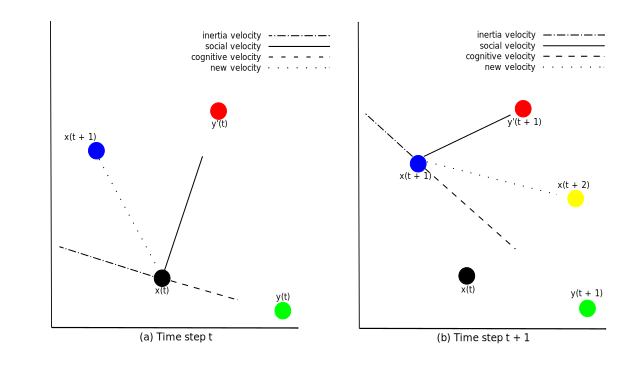
\includegraphics[width=4.5in,height=2.5in]{./pictures/geovelocity.pdf}}
	\caption{Visual particle velocity update \cite{SOSwarm,FundamentalSwarm,CompuIntelligenceIntro,PSOSelfHierarch}}
	%A Particle Swarm Algorithm for Symbols Detection in Wideband Spatial Multiplexing Systems --- Particle movement diagram

	\label{fig:particleVelocityUpdate}
	\end{center}
\end{figure}

As discussed in the PSO algorithm overview pbest is the best position the particle has occupied since the start of the algorithm. In the literature there are two defined methods of determining gbest. The most common method used is where gbest is the best position obtained by a particle in the swarm since the start of the algorithm. Thus long term knowledge dictates the best position found which favours exploitation \cite{CompuIntelligenceIntro,FundamentalSwarm}.

With the second method of determining the gbest is the best particle position occupied by any particle in the swarm in the \emph{current} iteration of the algorithm. Thus, short term knowledge dictates the best position found which favours exploration \cite{CompuIntelligenceIntro,FundamentalSwarm}.

As can be observed in equation (\ref{eq:velocityupdate}) the new velocity is added to the old velocity. Therefore, the velocity of particle can get very large, especially for those particles that are far from the pbest and gbest positions. Large velocities are necessary for early exploration, but if the velocity gets too large, the rate at which the particle moves in the solution space is to high and good solutions might be missed \cite{FundamentalSwarm}.

Thus, the velocity of a particle needs to be clamped to ensure it step size stays within acceptable bounds. Equation (\ref{eq:velocityclamp}) is used to clamp the velocity of a particle \emph{before} its position is updated \cite{FundamentalSwarm}.
\begin{align}
	v_i(t+1) &=
	\begin{cases}
	v'_i(t+1), &\text{if $v'_i(t+1) < V_{max}$}\\
	V_{max}, &\text{if $v'_i(t+1) \geq V_{max}$}
	\end{cases} \label{eq:velocityclamp}\\
	V_(max) &= \delta(x_{max} - x_{min})
\end{align}
Where $V_{max}$ is the maximum allowed velocity and $\delta \in (0,1]$. The values $x_{max}$ and $x_{min}$ are the respective minimums and maximums of the domain the algorithm is being applied to \cite{FundamentalSwarm}. The value of $\delta$ is very problem dependent and must be carefully chosen as to maximise the exploration - exploitation trade off \cite{FundamentalSwarm}. 

Most of the literature has concentrated on the velocity of the particle as a focal point because it is the main function performing the optimization. In research done by Ratnaweera et. al.\cite{PSOSelfHierarch} a particle positions in the solutions space are continually monitored. If the particle appears to be stagnant in the solution space, the velocity is first updated, and then the particle is reinitialized with a random position. The new position of the particle is then updated with the new velocity. Thus knowledge of the previous discarded particle is retained by using the velocity it had\cite{PSOSelfHierarch}.

In research done by Kalivarapu et al. \cite{PSOPheromones} a PSO algorithm is developed that seeks to incorporate the pheromone notion of ACO algorithms into the velocity updating of particles. The premise of the method is to allow greater sharing of information about promising areas between particles. The algorithm developed by the authors achieved promising results with the algorithm in certain cases finding solutions faster and better solutions than other PSO algorithms \cite{PSOPheromones}. 

Other research done by Monson and Seppi \cite{adaptPSO} is more concerned with how particle presented. In the general PSO algorithm, particles have no physical form or volume, thus particles in the swarm move through each other. The authors changed this in their algorithm by letting each particle have a radius around itself. Therefore, as particles move through the solution space and another particle at a certain time step occupies the same space, the particles are said to collide. As one would expect, when a collision occurs both particles are deflected into random directions \cite{adaptPSO}. At a greater expense of computational time due to constant collision detection, the PSO gains greater exploration in the solution space. 

Finally, in the research by Lenin and Monan a PSO algorithm is developed that is called the Attract and Repulse PSO (ARPSO). The algorithm continually monitors the solutions in the swarm. If the algorithm picks up that a certain percentage of the swarm is stagnating, the algorithm activates the repulse state. In the repulse state particle are repelled from other particles in the swarm, this facilitates greater exploration. After a certain number of iterations, the algorithm returns to its default state, where particles attract each other. The state of attraction facilitates exploitation \cite{PSOAttractRepulse}.
\subsubsection{Inertia Weight}
As an object moves with a certain velocity it carries momentum, if the object were to suddenly change direction, momentum would for a certain period still move the article in the previous direction. Inertia weight seeks to add type of behaviour to the particles of the PSO algorithm. It was initially developed to negate the use of clamping a particle velocity. The velocity update equation with added inertia is formulated in equation (\ref{eq:inertia}) \cite{FundamentalSwarm}.
\begin{equation}
v_i(t+1) = wv_i(t) + c_1\phi_{1}(t)[pbest - x_i(t)] + c_2\phi_{2}(t)[gbest - x_i(t)]\label{eq:inertia}
\end{equation}
The addition of inertia ($w$ in equation (\ref{eq:inertia}) to the general velocity update equation is simple and elegant which is why it has been adapted to a wide variety of PSO algorithms. The inertia value allows one to control the amount of control the social and cognitive components have with regard to velocity updates \cite{FundamentalSwarm}. 

For values of $w$ that are greater than 1, a large amount of momentum is preserved as the particles velocity are updated and hence, the particle explores more \cite{FundamentalSwarm}. When $w < 1$, each time the particle updates it velocity is loses a certain amount of momentum, hence, the particle seems to slow down allowing it to exploit the current solution space in finer detail \cite{FundamentalSwarm}.

Even though inertia was developed to remove the use of velocity clamping, it did not entirely achieve its goal. For values of $w$ that are greater than 1, the particle keeps a lot of momentum and accelerates even more. Therefore, as the particle accelerates its step size through the solution space gets larger and larger, increasing the probability that it will miss a good solution. This disadvantage is only applicable for algorithms that keep the inertia value static \cite{CompuIntelligenceIntro,FundamentalSwarm}.

To allow for a greater trade-off between exploration and exploitation, the inertia value was made dynamic. Exploration is favoured early on in an optimization algorithm and in return exploitation is favoured later on the algorithm when it is near an optimum. Thus, various methods linear decreasing and non-linear decreasing and have been developed that modify the inertia component as the algorithm moves around in the solution space \cite{CompuIntelligenceIntro,FundamentalSwarm}.

Finally, a similar inertia type component was developed from the analyse of particle dynamics \cite{FundamentalSwarm}. This new component is called the \emph{constriction coefficient} and like the inertia above, also modifies the velocity update equation slightly\cite{adaptPSO,FundamentalSwarm,CompuIntelligenceIntro}. 

This modification can be observed in equation (\ref{eq:velocityconstriction}), which is the standard velocity equation with the constriction coefficient. The constriction coefficient is formulated in equation (\ref{eq:constriction})\cite{adaptPSO,FundamentalSwarm,CompuIntelligenceIntro}.
\begin{align}
v_i(t+1) &= \chi[v_i(t) + c_1\phi_{1}(t)[pbest - x_i(t)] + c_2\phi_{2}(t)[gbest - x_i(t)]]\label{eq:velocityconstriction}\\
\chi &= \frac{2\kappa}{\lvert 2 - \phi - \sqrt{\phi^2 - 4\phi}\rvert}\label{eq:constriction}
\end{align}

The constriction coefficient is represented by the value $phi$ and allows one to omit the usage of velocity clamping. The constriction coefficient evaluates to an ever decreasing value between $[0,1]$. By using the constriction coefficient the PSO algorithm is also guaranteed to converge for values of $phi \geq 4$ and $\kappa \in [0,1]$. As with the inertia discussed above, high values of $\kappa$ allows for greater exploration and slow convergence. Where as low values of $\kappa$ forces the algorithm to exploit the solution space and converge quickly \cite{adaptPSO,FundamentalSwarm,CompuIntelligenceIntro}.
\subsection{PSO on the FAP}
\label{sec:psoonfap}
The PSO algorithm is also a relatively new algorithm and has been applied to only a handful of NP-Complete problems that includes the FAP. In this dissertation the PSO algorithm will be utilized on the FS-FAP to try and produce optimal solutions. 

In the literature only two groups have presented research where the PSO has been applied on the FAP to produce a near optimal solution. The research presented by these groups concentrate on the MS-FAP variant of the FAP. Thus, the aim of their algorithm is to reduce the span of frequencies used, where as the problem this dissertation is concerned with is the FS-FAP where the amount of interference generated needs to be minimized. 

To date, no PSO algorithm has been presented which has been designed to operate on the FS-FAP variant of the FAP. Therefore, the interest in the research presented is more to do with how the authors went about encoding a particular frequency plan as a position for a particle, than with the actual optimization procedure.

A general overview of the work produce by these groups will now be presented.

In the research presented by Elkamchouchi et. al\cite{EgyptFAPPSO} a PSO algorithm is applied to produce optimal solutions for the MS-FAP. The way the authors went about to assign frequencies in their algorithm is known as the Frequency Exhaustive Assignment (FEA).
This method works by first generated a list of calls, called a \emph{call list} denoting calls that occur in the system\cite{EgyptFAPPSO}. 

The method then iterates over the calls in the list and assigns the lowest possible frequencies to the calls without violating interference constraints\cite{EgyptFAPPSO}. The authors note that the specific frequency that is assigned to a particular call depends heavily on the order the calls are in the list\cite{EgyptFAPPSO}.

As can be observed from the above discussion, the PSO has been successfully applied to the FAP. The particular variant of the FAP was the MS-FAP and also the authors PSO is tasked with minimizing constraint violations.

With the success of the PSO on the MS-FAP, for this dissertation the PSO algorithm was selected as the primary means by which to address the FAP. In addition to the successful application of the PSO to the FAP other factors also influenced the final decision to utilize the PSO instead of another algorithm.

The PSO algorithm is short and elegant. As discussed in the overview of the PSO, the algorithm utilizes the "flying" approach to search the problem space. With this approach one point progressively move towards another. Using this approach, the algorithm able to adequately explore the problem space much more thoroughly.

The algorithm also makes extensive use of knowledge gained by the various particles as the search the problem space. Not only does each particle keep personal history (with pbest) but the swarm as a whole keeps a history of the best particle with (with gbest). Thus, with regard to FAP, it is possible that even though a particle might be in a overall bad position, it might have some small bit of good knowledge being overshadowed by bad knowledge. Through the extensive use of historic knowledge good information is more likely to be shared or kept slightly longer in the algorithms collective knowledge.

For this dissertation the PSO will applied to the FS-FAP and thus the approach as used in by the authors in the above literature cannot be used. FS-FAP is concerned with interference generated and there are some constraints which cannot be broken, where the MS-FAP the performance measure is explicitly the amount of constraints violated.

The PSO algorithm might be short and elegant, but applying it the FS-FAP requires various new techniques in response to the following questions
\begin{itemize}
\item How to best represent a particle as a frequency plan ?
\item How to ``fly'' one frequency plan to another ?
\item How to avoid particles using forbidden frequencies when they fly towards a particular plan ?
\end{itemize}

The above questions are only the preliminary questions and are in fact problem that must be addressed for a successful application of the PSO to the FAP. In chapter~\ref{chpt:psoapplicationFAP} a discussion will be presented on how these problems were solved as well as how other problems were solved that were not anticipated.

In this section a discussion was presented which discussed literature that utilized the PSO on the FAP. Furthermore, it was formally stated that the PSO would be the primary algorithm in this dissertation to be applied to the FAP.

This section concludes the discussion on the PSO as well as the Swarm Intelligence chapter. In the following section a summary is presented on this chapter.
\section{Summary}
In this chapter a discussion was given on three swarm intelligence algorithms. The first section presented a discussion on the Ant Colony Optimization Algorithm.

The general flow of the algorithm was presented with the help of a diagram (see figure \ref{fig:ACOAlgorithmFlowChart}) as well as an explanation with regard to how the algorithm came about and the basic flow of the algorithm. The defining characteristics of the algorithm were also discussed. The discussion on the ACO algorithm concluded with a literature review of the ACO being applied to the FAP.

The second section that was presented provided an overview of the Artificial Bee Colony Optimization Algorithm. A discussion was presented on how the algorithm was developed and how the algorithm performs its search in a problem space. A diagram was also presented that outlines the general flow of the ABC algorithm.

Also within the second section, a series of defining characteristics are presented and explained. Each characteristic is a defining attribute of the algorithm that makes it unique with regard to other algorithms. No literature study was presented on the algorithm being applied on the FAP since to date; no research has been presented of such an ABC algorithm.

This chapter concluded with a discussion on the most important algorithm. The algorithm this dissertation will be using to apply it to the FAP, namely the Particle Swarm Optimization algorithm. In the last section how the algorithm was developed was discussed as well as the general flow of the algorithm when search the problem space.

A diagram depicting the flow of the PSO algorithm was also presented (see figure \ref{fig:PSOAlgorithmFlowChart}). Furthermore, characteristics that make the algorithm unique were explained. The final section of this chapter concluded with a literature review of the PSO algorithm being applied to the FAP.
%Swarm Intelligence
\chapter{PSO on benchmark functions}
\label{chpt:benchmark}
\section{Introduction}
In this section a discussion will be presented on a series of optimisation benchmark functions. First a formulation of all the benchmark functions will be given. In the second section all the benchmark functions will be plotted on a 3d graph. Finally this chapter will conclude with a presentation of the results obtained by the PSO algorithm.

The functions vary from being relatively easy to optimize, to functions that contain lots of local minima and a slightly concealed global minima. In total fourteen benchmark functions will be formulated and benchmarked againts.

If one observed the following research \cite{devparallelgasa,CompuIntelligenceIntro,FundamentalSwarm}. Various optimisation algorithms are benchmarked such as Genetic Algorithm, Artificial Bee Colony algorithm, Tabu Search and Simulated Annealing. In the presented research the algorithms are benchmarked using numerical optimization functions.

Numerical optimization functions are good candidates to test optimisation algorithms as with a few slight changes the function operates in more dimensions or can have more or less optima\cite{devparallelgasa,CompuIntelligenceIntro,FundamentalSwarm}. Being able to alter these functions is a desirable trait as it enables one to accurately benchmark an algorithm, not only with regard to how the algorithm coupes with increased dimensionality but also in the algorithms accuracy in locating optima\cite{devparallelgasa,CompuIntelligenceIntro,FundamentalSwarm}.

The reason why these functions have variable amount of local and global optima, it to test various factors on how good the algorithm is that is being applied on the function. The factors that are tested are\cite{CompuIntelligenceIntro,FundamentalSwarm}:
\begin{itemize}
\item Rate of convergence
\item Exploration
\item Exploitation
\item Diversity
\item Breaking out of local minima
\item Information sharing
\end{itemize}

As discussed previously the numerical functions have predetermined optima, which means researchers are able to produce statistical information on how the algorithm performs. For instance, researchers will not be able to measure accurately the performance of the algorithm on a NP-Complete problem\cite{CompuIntelligenceIntro,FundamentalSwarm}. Yes, they can compare results with what other algorithms have produced, but cannot with absolute certain say or measure the algorithm convergence, diversity etc. on NP-Complete problems as their problem spaces are huge\cite{evalevoalgo}. 

With these benchmark functions, the optima have been mathematically calculated and their position is known within the problem space\cite{evalevoalgo}. Thus, researchers can now with surety measure the convergence rate, diversity and compare it with other algorithms, since the domain the algorithms operate it is not as specific as a NP-Complete problem\cite{evalevoalgo}. Rather, the domain is mathematical and deterministic and therefore allows easy comparison\cite{evalevoalgo}.

In this dissertation, two PSO algorithm were developed specifically to measure the performance of the PSO algorithm and also to better understand the various underlying dynamics of the algorithm.

The first PSO that was developed was just the standard PSO algorithm with no constriction coefficient or inertia weight. The second PSO algorithm differed to the standard algorithm in the sense that it utilizes the notion of inertia to move particles. 

Both of these algorithms have been applied to all fourteen benchmarks that are presented in the chapter and will be compared (where applicable) to other optimisation algorithms that have also been applied to the same benchmark problems. The comparison between these algorithms will be presented in section~\ref{sec:benchResults}.

In the next section, all the benchmarks that will be used for testing the PSO algorithms will be formulated. For the interested reader, 3D graphs along with the python code that generated the graphs are presented in the appendix. This chapter will conclude with a section on the results of the PSO algorithms that were developed being applied to the presented benchmarked as well as compared with other results that have been obtained by other algorithms and presented in the literature.
\section{Test Functions}
In this section all the test functions on which the two developed PSO algorithms will be benchmarked against will be presented. For each test function that is presented a mathematical formulation will be given and the global optimum will be explicitly stated. In addition to the formulation and global optimum, each function will also be classified whether it is a unimodal or modal function as well as whether it is separable or non-separable. Each of these classifications will now be explained.

\begin{description}
\item{\textbf{Unimodal}} --- A particular problem is classified as being unimodal when there is only clear solution. With only one clear solution, it means there is only one global optimum point in the solution space\cite{evalevoalgo,numericalABC,FundamentalSwarm,CompuIntelligenceIntro}.
\item{\textbf{Multimodal}} --- A problem is multimodal when it has more than one defined solution. Thus, the particular problem space contains multiple global optima\cite{evalevoalgo,numericalABC,FundamentalSwarm,CompuIntelligenceIntro}.
\item{\textbf{Separable}} --- Functions that are classified as being separable have the characteristic when the function can be written as a series of summations of just one variable\cite{numericalABC}. This quality makes the function easier to solve as the algorithm has only one variable to be concerned about\cite{evalevoalgo,numericalABC}. Separable functions also have the inherent quality of being scalable, meaning they can be easily be adapted to higher dimensions\cite{evalevoalgo,numericalABC}.
\item{\textbf{Non-separable}} --- Functions classifiied as non-separable cannot be rewritten into a series of summation functions as the variables used in the functions have the characteristic of being interrelated\cite{evalevoalgo,numericalABC}. The interrelation of the variables makes non-separable functions more difficult than separable functions to solve since the algorithm has more interdependent variables to be concerned with\cite{evalevoalgo,numericalABC}.
\end{description}

The De Jong test functions (F1, Shekel's Foxhole) are not considered to be the gold standard of testing optimisation algorithms\cite{evalevoalgo}. The only reason for their extensive use in the literature is due to the functions being the first to be developed and applied to test an optimisation algorithm i.e. Genetic Algorithm\cite{devparallelgasa,evalevoalgo}.

Since the inception of the De Jong test functions, additional functions have been developed which make it more difficult for an optimisation algorithm to locate the optimum\cite{evalevoalgo}. These functions are more difficult in the sense, as they have multiple local optima, which does in actual fact leads the algorithm astray which is to say the problem space is deceptive\cite{CompuIntelligenceIntro,FundamentalSwarm,evalevoalgo}. 

Problems that have deceptive search spaces tests how good the algorithm is resistant to Hill-climbing\footnote{continously selecting what seems to be better moves, but in reality its moving towards a local optima peak} and hence how efficient the algorithm is in exploring the entire search space\cite{evalevoalgo}.
%\textbf{Development of a parallel optimization method based on genetic simulated annealing algorithm}\\
%\textbf{Adaptive Diversity in PSO}\\
%\textbf{A hybrid intelligent genetic algorithm}\\
%\textbf{A Diversity-Guided Particle Swarm Optimizer – the ARPSO}\\
%\textbf{A distributed hierarchical genetic algorithm for efficient optimization and pattern matching}\\
%\textbf{Tabu search for global optimization of continuous functions with application to phase equilibrium calculations}\\
%\textbf{Tabu Search applied to global optimization}\\
%\textbf{On the performance of artificial bee colony (ABC) algorithm}\\
%\textbf{Improving solution characteristics of particle swarm optimization using digital pheromones}\\
%\textbf{Continuous ant colony system and tabu search algorithms hybridized for global minimization of continuous multi-minima functions}\\
%\textbf{Chaotic bee colony algorithms for global numerical optimization}\\
%\textbf{A powerful and efficient algorithm for numerical function optimization: artificial bee colony (ABC) algorithm}\\
%\textbf{A New Quantum Behaved Particle Swarm Optimization}\\
%\textbf{A comparative study of Artificial Bee Colony algorithm}\\
\subsection{DeJong F1 Function}
\begin{equation}
\label{eq:DeJongF1}
	f(x) = \sum_{i=1}^n x^2_i, -5.12 \leq x_i \geq 5.12, i \in \mathbb{N}
\end{equation}
The DeJong F1 Function has the following global minimum when $f(x) = 0, x(i) = 0, i:n$ where $n$ is the amount of dimensions\cite{numericalABC,ABCCompareStudy,ARPSO,PerfABC,ContinACSTS,TestFunctions}. In the literature the function is classified as being unimodal and separable\cite{ABCCompareStudy,TestFunctions}. 
\subsection{Shekel's Foxhole}
\begin{align}
\label{eq:shekel}
	f(x_1,x_2) &= \{0.002 + \sum^{25}_{j=1} [j + (x_1 - a_{1j})^6 + (x_2 - a_{2j})^6]^{-1}\}^{-1}\\
\intertext{where}
	a &= \begin{pmatrix} \nonumber
			-32 & -16 & 0 & 16 & 32 & -32 & ... & 0 & 16 & 32 \\
			-32 & -32 & -32 & -32 & -32 & -16 & ... & 32 & 32 & 32 \\
		 \end{pmatrix}
\end{align}
the variables $x_1$ and $x_2$ are usually restricted to the square represented by $-65.356 \leq x_1 \leq 65.357, -65.357 \leq x_2 \leq 65.356$\cite{ABCCompareStudy,TSGlobalOptimization,ContinACSTS,TestFunctions}. The global optimum is when $f(x_1,x_2) = 0, \{x_1,x_2\} = \{-32,-32\}$\cite{ABCCompareStudy,TSGlobalOptimization,ContinACSTS,TestFunctions}.

The matrix controls the holes that appear in the search space. The interested reader is directed to the 3D graph rendering of this function presented in the appendix on page~\pageref{fig:ShekelGraph} for a visual representation. In the literature the function is classified being multimodal and separable\cite{adaptPSO,ABCCompareStudy,TestFunctions}.
\subsection{Rastrigin}
\begin{equation}
	f(x) = 10n + \sum_{i=1}^n [x_i^2 - 10\cos(2 \pi x_i)],\, i \in \mathbb{N}
\end{equation}
The values of the variable $x_i$ is bounded by the hypercube $-5.12 \leq x_i \leq 5.12$\cite{adaptPSO,ABCCompareStudy,numericalABC,ARPSO,PerfABC,HybridIntelliGA,TestFunctions}. The global optimum for the function is when $f(x_i) = 0,\, x_i = 0, \, i = 1,\dots,n$\cite{adaptPSO,ABCCompareStudy,numericalABC,HybridIntelliGA,TestFunctions}.

Rastrigins function is based on DeJong's first function equation~\ref{eq:DeJongF1} adding a cosine term, which in turns alters the problem space by introducing many local minima\cite{numericalABC,PerfABC,HybridIntelliGA,TestFunctions}. In the literature the function is classified being multimodal and separable\cite{adaptPSO,ABCCompareStudy,numericalABC,ARPSO,ChaoticABC,PerfABC,HybridIntelliGA,TestFunctions}.
\subsection{Schwefel}
\begin{equation}
	f(x) = 418.9829n - \sum^n_{i=1} [x_i\sin{\sqrt{|x_i|}}], \qquad i \in \mathbb{N}
\end{equation}
The variable $x_i$ is restricted to be in the hypercube $-500 \leq x_i \leq 500, i = 1,\ldots,n$\cite{ABCCompareStudy,numericalABC,HybridIntelliGA,DistributedHierarchicalGA,TestFunctions}. The global optimum for the function is $f(x) = 0$ when $x_i = 420.9687$\cite{ABCCompareStudy,numericalABC,HybridIntelliGA,DistributedHierarchicalGA,TestFunctions}. 

If one observes the 3D rendering of the schwefel function problem space on page~\pageref{fig:SchwefelGraph}, one can see that the search space contains a great number of peaks which might be local optima. The function also has the characteristic of having a second best optima far from the global optima which many algorithms get trapped in\cite{ABCCompareStudy,numericalABC,HybridIntelliGA,DistributedHierarchicalGA,TestFunctions}. In the literature the function is classified as being multimodal and separable\cite{ABCCompareStudy,numericalABC,HybridIntelliGA,TestFunctions}.
\subsection{Griewank}
\begin{equation}
	f(x) = \sum^n_{i=1} \frac{x^2_i}{4000} - \prod^n_{i=1}\cos{(\frac{x_i}{\sqrt{i}})} + 1, \qquad i \in \mathbb{N}
\end{equation}
The variable $x_i$ is bounded to within the hypercube $ -600 \leq x_i \leq 600 $\cite{numericalABC,ABCCompareStudy,ARPSO,PerfABC,ContinACSTS,TestFunctions}. The global optimum of the function is when $f(x) =0$ which occurs when $ x_i = 0, i = 1, \dots, n $\cite{numericalABC,ABCCompareStudy,ARPSO,PerfABC,ContinACSTS,TestFunctions}.

As with the schwefel function, the Griewank function also has a great number of peaks and valleys which many algorithm get trapped in. A particular quality of the griewank function is at low dimensions, the function is quite difficult to solve, whereas it has been shown that at higher dimensions the function becomes much easier due to there being less peaks and valleys to navigate in the search space\cite{evalevoalgo,ABCCompareStudy,numericalABC,PerfABC,TestFunctions}. In the literature the function is classified as being multimodal and non-separable\cite{adaptPSO,ABCCompareStudy,numericalABC,ChaoticABC,PerfABC,TestFunctions}.
\subsection{Salomon}
\begin{equation}
	f(x) = -\cos{(2\pi\sum_{i=1}^n\sqrt{x_i^2})} + 0.1 \sqrt{\sum_{i=1}^n x_i^2} + 1, \quad i \in \mathbb{N}
\end{equation}
Unlike the previous functions discussed in this section, the Salomon function imposes no constraint on the $x_i$ variable. The global optimum is when $f(x) = 0$ and $x_i = 0$ where $i = 1,\ldots,n$. This particular function seems to have been applied as benchmarking function yet, as no literature can be found. Nonetheless, the function is indeed a numerical optimisation function that is classified as being multimodal and non-separable\cite{http://www.it.lut.fi/ip/evo/functions/node12.html}.
\subsection{Ackley}
\begin{equation}
	f(x) = -20e^{-0.2\sqrt{\frac{1}{2}\sum_{i=1}^n x_i^2}} - e^{\frac{1}{2}\sum_{i=1}^n\cos{2\pi x_i}} + 20 + e^1, \qquad i \in \mathbb{N}
\end{equation}
The variable $x_i$ is restricted to the hypercube represented by $-32.768 \leq x_i \leq 32.768$\cite{numericalABC,ABCCompareStudy,ARPSO,TestFunctions}. The global minimum is when $f(x) = 0$ and is obtainable for $x_i = 0, i = 1,\ldots,n$\cite{numericalABC,ABCCompareStudy,ARPSO,TestFunctions}.

As can be observed from the mathematical formulation of the function, the function utilizes a exponential term. By using the exponential term the problem space contains numerous local optima which requires an algorithm to search much wider to avoid getting trapped. The literature classifies this function as being multimodal and non-separable\cite{adaptPSO,ABCCompareStudy,numericalABC,TestFunctions}.
\subsection{Six-Hump Camel Back}
\begin{equation}
	f(x_1,x_2) = (4 - 2.1x_1^2 + x_1^{\frac{4}{3}})x_1^2 + (x_1x_2) + (-4 + 4x_2^2)x_2^2
\end{equation}
The variables $x_1$ and $x_2$ are subject to the following boundary constraints $-3 \leq x_1 \leq 3$ and $-2 \leq x_2 \leq 2$\cite{DistributedHierarchicalGA,TestFunctions}. The global minimum is when $f(x_1,x_2) = -1.0316$ and is obtained when $x_1 = -0.0898$ and $x_2 = 0.7126$ or when  $x_1 = 0.0898$ and $x_2 = 0.7126$\cite{DistributedHierarchicalGA,TestFunctions}. 

True to its name the function has six peaks, four of which are local minima and two that are global minima as has already been defined. The literature classifies this function as being multimodal and non-separable\cite{ABCCompareStudy,TestFunctions}.
\subsection{Shubert}
\begin{equation}
	f(x_1,x_2) = -\sum_{i = 1}^5 (i\cos{(i +1)x_1 + 1})\sum_{i=1}^5 (i\cos{(i+1)x_2 + 1})
\end{equation}
The search domain is constrained to $-10 \leq x_i \leq 10, i = 1,2, \ldots, n$\cite{ABCCompareStudy,TSGlobalOptimization,ContinACSTS,TestFunctions}. The global optimum which is when $f(x_i) = -186.7309$\cite{ABCCompareStudy,TSGlobalOptimization,ContinACSTS,TestFunctions}. 

As can be observed from the 3D graph presented in the appendix on page~\pageref{fig:ShubertGraph} the landscape of the Shubert function contains various peaks and slopes. Thus, the function is classified as being multimodal and non-separable\cite{ABCCompareStudy,TestFunctions}.
\subsection{Himmelblau}
\begin{equation}
	f(x_1,x_2) = (x_1^2 + x_2 - 11)^2 + (x_1 + x_2^2 - 7)^2
\end{equation}
The variables $x_1,x_2$ are constraint to be within the hypercube represented by $-6 \leq x_1 \leq 6, -6 \leq x_2 \leq 6$\cite{TestFunctions,ABCCompareStudy}. The Himmelblau function contains no local optima, but on the contrary, it has 4 global optima when $f(x_i) = 0$ which can be obtained at the following points\cite{TestFunctions,ABCCompareStudy}.
\begin{itemize}
\item $(x_1,x_2) = (-3.779310,-3.283185)$
\item $(x_1,x_2) = (-2.805118,3.131312)$
\item $(x_1,x_2) = (3,2)$
\item $(x_1,x_2) = (3.584428,-1.848126)$
\end{itemize}
The literature classifies the function as being multimodal and non-separable\cite{TestFunctions,ABCCompareStudy}.
\subsection{Rosenbrock Valley}
\begin{equation}
	f(x) = \sum_{i=1}^{n-1}[100(x_{i+1} - x_i^2)^2 + (1-x_i)^2
\end{equation}
The variable $x_i$ is bounded to with the following constraint $ -2.048 \leq x_i \leq 2.048 $\cite{numericalABC,ABCCompareStudy,ARPSO,PerfABC,TSGlobalOptContinFunc,HybridIntelliGA}. The global optimum is when $f(x) = 0$ and is obtained when $x_i = 1, i = 1,\ldots,n$\cite{numericalABC,ABCCompareStudy,ARPSO,TSGlobalOptContinFunc,HybridIntelliGA}.

The rosenbrock search space has a curving valley which leads forces algorithms to coupe with the changing direction of the landscape\cite{numericalABC,ABCCompareStudy,ChaoticABC,PerfABC,HybridIntelliGA}. If the algorithm does not adapt to the changing direction it will fail in locating the global optimum. The function is classified as being multimodal and non-separable\cite{numericalABC,ABCCompareStudy,ChaoticABC,PerfABC,HybridIntelliGA}.
\subsection{Dropwave}
\begin{equation}
	f(x) = -\frac{1 + \cos{(12\sqrt{x_1^2 + x_2^2})}}{\frac{1}{2}(x_1^2 + x_2^2) + 2}
\end{equation}
The variables $x_1$ and $x_2$ are restricted to be within the following bounds $-5.12 \leq x_i \leq 5.12$\cite{TestFunctions}. The landscape of this function resembles that of a droplet falling into a pool of water, as can be observed from the 3D graph presented in the appendix on page~\pageref{fig:DropwaveGraph}. Due to its ``wave'' nature, the function has various local minima and only a single optima which is when $f(x_1,x_2) = 0$. The function is classified being multimodal and non-separable\cite{TestFunctions}.
\subsection{Easom}
\begin{equation}
	f(x_1,x_2) = -\cos(x_1)\cos(x_2)e^{(-(x_1 - \pi)^2 - (x_2 - \pi)^2)}
\end{equation}
The variables $x_1$ and $x_2$ are restricted to be within the hypercube represented by $-100 \leq x_1 \leq 100, -100 \leq x_2 \leq 100$\cite{TSGlobalOptContinFunc,ContinACSTS,TestFunctions}. The global minimum is when $f(x_1,x_2) = -1$ and is obtainable if $(x_1,x_2) = (\pi,\pi)$\cite{TSGlobalOptContinFunc,ContinACSTS,TestFunctions}. 

The easom function has a deceptive global minimum as it is very close to other local minima\cite{ABCCompareStudy,TSGlobalOptimization}. As can be observed from the 3D graph of the function on page~\pageref{fig:EasomGraph}, the search space is a flat with the global minima clearly visible. Flat search spaces are difficult to navigate by algorithms as the surrounding area gives no indication whether the algorithm is on the right track of not. The function is classied as being multimodal and non-separable in the literature \cite{ABCCompareStudy,TSGlobalOptimization,TSGlobalOptContinFunc}.
\subsection{Branins}
\begin{align}
	f(x_1,x_2) &= a(x_2 - bx_1^2 + cx_1 - d)^2 + e(1-f)\cos{x_1} + e \\
\intertext{where}
	a &= 1\nonumber\\
	b &= \frac{5.1}{4\pi^2}\nonumber\\
	c &= \frac{5}{\pi}\nonumber\\
	d &= 6\nonumber\\
	e &= 10\nonumber\\
	f &= \frac{1}{8\pi}\nonumber
\end{align}
The variables $x_1$ and $x_2$ are subject to the following boundary constraints $-5\leq x_1 \leq 10, 0 \leq x_2 \leq 10$\cite{ABCCompareStudy,TSGlobalOptimization,ContinACSTS,TestFunctions}. The global optimum is when $f(x_1,x_2) = 0.397887$ and is obtainable when $x_1$ and $x_2$ have the following values\cite{ABCCompareStudy,TSGlobalOptimization,ContinACSTS,TestFunctions}:
\begin{enumerate}
\item $x_1 = -\pi,\:x_2=12.275$
\item $x_1 = \pi,\:x_2=2.275$
\item $x_1 = 9.42478,\:x_2=2.475$
\end{enumerate}
The literature classifies this function as being multimodal and separable\cite{ABCCompareStudy,TSGlobalOptimization,ContinACSTS,TestFunctions}.
\subsection{Michalewicz}
\begin{equation}
	f(x) = -\sum_{i=1}^n\sin{(x_i)}[\sin{(\frac{(1 - x_i^2)}{\pi})}]^{2m}, \qquad i,m \in \mathbb{N}
\end{equation}
The variable $x_i$ is usually constricted to the following defined boundary $0 \leq x_i \leq \pi, i = 1,\ldots,n$\cite{ABCCompareStudy,TestFunctions}. The parameter $m$ defines the steepness of the valleys in the function. The function has two approximated global minima's that are difficult to locate since their size in comparison to the rest of the search space is relatively small\cite{ABCCompareStudy,TestFunctions}.
%http://www.geatbx.com/docu/fcnindex-01.html#P216_11735
\begin{enumerate}
\item $f(x) = -4.687,\: n = 5$
\item $f(x) = -9.66,\: n = 10$
\end{enumerate}
In the literature the function is classified as being multimodal and separable\cite{ABCCompareStudy}.
\subsection{Goldstein}
\begin{align}
	f(x_1,x_2) &= (1 + (x_1 + x_2 + 1)^2)\nonumber\\
			   &=*(19-14x_1+3x_1^2 -14x_2 + 6x_1x_2 + 3x_2^2)\nonumber\\
			   &=*(30 + (2x_1 -3x_2)^2\nonumber\\
			   &=*(18 - 32x_1 + 12x_1^2 +48x_2 -36x_1x_2 + 27x_2)\nonumber
\end{align}
The variables $x_1$ and $x_2$ are subject to the following boundary constraints $-2 \leq x_1 \leq 2, -2 \leq x_2 \leq 2$\cite{ABCCompareStudy,TSGlobalOptimization,TSGlobalOptContinFunc,ContinACSTS,TestFunctions}. The function has only one global minimum four local optima\cite{ABCCompareStudy,TSGlobalOptimization}. The global optimum is when $f(x_1,x_2) = 3$ and is obtainable when $x_1 = 0$ and $x_2 = -1$\cite{ABCCompareStudy,TSGlobalOptimization,TSGlobalOptContinFunc,ContinACSTS,TestFunctions}.

The literature classifies this function as being multimodal and non-separable\cite{ABCCompareStudy}.

\section{Results}
\label{sec:benchResults}
In the previous section sixteen benchmark functions were mathematically defined, where applicable comments were given on the search space. For each function the following was explicitly stated:
\begin{itemize}
\item The global optimum and where is located.
\item Whether the function is unimodal or multimodal.
\item Whether the function is non-separable or separable.
\end{itemize}
In this section the results will be presented of how the two PSO algorithms that were developed performed on each of the presented benchmark functions. 

The algorithms will be compared with the following criteria on each benchmark.
\begin{itemize}
\item The number of iterations the algorithm took to find the global optimum
\item The accuracy of the algorithm, which means if the algorithm has indeed located the optimum or if not, how far off is the algorithm.
\item The PSO is a population-based algorithm, thus diversity is important. Diversity will be measured and compared on each benchmark function.
\end{itemize}
For each of the above criteria a subsection will be presented. Where possible the results obtained will be compared to other algorithms that have been applied to similar test functions.

\subsection{Fina values}
\begin{center}
	\begin{tabular}{| c | c | c | c | c | c |}
	\hline
	Function & PSO & PSO* & GA & TS & ABC\\  \hline
	DeJong F1 & 0 & -- & -- & -- & --\\ \hline
	Shekel's Foxhole & 0 & -- & -- & -- & --\\ \hline
	Rastrigin & 0.74622 & -- & N/A & N/A & N/A\\ \hline
	Schwefel & -1.19069e+43 & -- & N/A & N/A & N/A\\ \hline
	Griewank & 1.00003 & -- & N/A & N/A & N/A\\ \hline
	Salomon & -0.460561 & -- & -- & -- & --\\ \hline
	Ackley & -4.5901 & -- & N/A & N/A & N/A\\ \hline
	Six-Hump camelback & -1.03163 & -- & -- & -- & --\\ \hline
	Shubert & -186.731 & -- & -- & -- & --\\ \hline
	Himmelblau & 1.02103 & -- & -- & -- & --\\ \hline
	RosenbrockValley & 1.81101e-08 & -- & -- & -- & --\\ \hline
	Dropwave & 4.59843e-15 & -- & -- & -- & --\\ \hline
	Easom & -1 & -- & -- & -- & --\\ \hline
	Branins & 1.22875 & -- & N/A & N/A & N/A\\ \hline
	Michalewicz & -2.40391 & -- & -- & -- & --\\ \hline
	Goldstein & infinity & -- & -- & -- & --\\ \hline
	\end{tabular}
\end{center}
\subsection{Diversity}
\begin{center}
	\begin{tabular}{| c | c | c | c | c | c |}
	\hline
	Function & PSO & PSO* & GA & TS & ABC\\  \hline
	DeJong F1 & -- & -- & -- & -- & --\\ \hline
	Shekel's Foxhole & -- & -- & -- & -- & --\\ \hline
	Rastrigin & -- & -- & -- & -- & --\\ \hline
	Schwefel & -- & -- & -- & -- & --\\ \hline
	Griewank & -- & -- & -- & -- & --\\ \hline
	Salomon & -- & -- & -- & -- & --\\ \hline
	Ackley & -- & -- & -- & -- & --\\ \hline
	Six-Hump camelback & -- & -- & -- & -- & --\\ \hline
	Shubert & -- & -- & -- & -- & --\\ \hline
	Himmelblau & -- & -- & -- & -- & --\\ \hline
	RosenbrockValley & -- & -- & -- & -- & --\\ \hline
	Dropwave & -- & -- & -- & -- & --\\ \hline
	Easom & -- & -- & -- & -- & --\\ \hline
	Branins & -- & -- & -- & -- & --\\ \hline
	Michalewicz & -- & -- & -- & -- & --\\ \hline
	Goldstein & -- & -- & -- & -- & --\\ \hline
	\end{tabular}
\end{center}
\subsection{Accuracy}
\begin{center}
	\begin{tabular}{| c | c | c | c | c | c |}
	\hline
	Function & PSO & PSO* & GA & TS & ABC\\  \hline
	DeJong F1 & -- & -- & -- & -- & --\\ \hline
	Shekel's Foxhole & -- & -- & -- & -- & --\\ \hline
	Rastrigin & -- & -- & -- & -- & --\\ \hline
	Schwefel & -- & -- & -- & -- & --\\ \hline
	Griewank & -- & -- & -- & -- & --\\ \hline
	Salomon & -- & -- & -- & -- & --\\ \hline
	Ackley & -- & -- & -- & -- & --\\ \hline
	Six-Hump camelback & -- & -- & -- & -- & --\\ \hline
	Shubert & -- & -- & -- & -- & --\\ \hline
	Himmelblau & -- & -- & -- & -- & --\\ \hline
	RosenbrockValley & -- & -- & -- & -- & --\\ \hline
	Dropwave & -- & -- & -- & -- & --\\ \hline
	Easom & -- & -- & -- & -- & --\\ \hline
	Branins & -- & -- & -- & -- & --\\ \hline
	Michalewicz & -- & -- & -- & -- & --\\ \hline
	Goldstein & -- & -- & -- & -- & --\\ \hline
	\end{tabular}
\end{center}

\section{Summary}
In this chapter a series of mathimatical optimisation problems were presented. Each problem was mathematically formulated as well as categorised as to whether the particular problem is multi-modal and seperable.

To get a better idea on how the Particle Swarm Optimisation (PSO) algorithm operates and performs two PSO algortihms were developed. The first PSO algorithm uses the standard velocity equation with no alterations. The second PSO algorithm uses the notion of inertia with regard to velocity calculation.

The algorithms that were developed were tested on all the mathematical problems outlined at the start of this chapter. The chapter concluded with a presentation of the results obtained by the algorithms along with a short discussion on the obtained results.
%Swarm Intelligence and the Frequency Assignment Problem
\part{Implementation}
\bibliography{ReferenceDB}
\bibliographystyle{plain}
\end{document}
